% =====================================================================
%  Capitolo 13 — Git, componenti ed ereditarietà: la terza lezione di
%  programmazione con i Blueprint di Unreal Engine (Game Design, primo
%  anno)
%  Fonte: trascrizione della lezione GD13 (Game Design, primo anno),
%  terza lezione di programmazione, diretta prosecuzione dei capitoli 7
%  e 12. È la lezione "di lunedì" annunciata nel capitolo 12: la prima
%  parte è dedicata a Git e GitHub, la seconda torna ai Blueprint. Lezione
%  ibrida e poco affollata ("siamo in tre oggi"): una parte della classe
%  in aula, una parte (Federica, Daniele) collegata da remoto con lo
%  schermo condiviso sul canale vocale "GD1 Voice" di Discord.
%  Contenuti, nell'ordine della lezione: il problema dei file persi e il
%  version control; Git, GitHub e i concorrenti (Lore di Epic Games,
%  GitKraken, Sourcetree); il limite dei 100 MB, Git LFS e i server
%  propri; il primo repository (privato, con il .gitignore di Unreal);
%  GitHub Desktop e il clone; il setup di un progetto Unreal dentro la
%  cartella del repository; commit e push; i collaboratori; fetch e pull
%  a engine chiuso; la history che non dimentica nulla; i conflitti; i
%  branch (per persona, per feature, release, alpha, beta) e il merge;
%  le mappe come fonte di conflitti e i sub-level; la history come prova
%  di chi ha lavorato; Discard Changes e il branch da un commit vecchio;
%  il riepilogo del task per chi era assente; i plugin (Text 3D, le due
%  cartelle dei plugin, il plugin da non disattivare); il vecchio input
%  system (Action e Axis Mappings); i componenti (Actor Component e
%  Scene Component, l'Health Component, la Damage Area); le funzioni
%  (input, output, funzioni pure, Collapse to Function, il limite dei
%  nodi latenti); la Game Instance (Event Init, Maps & Modes, il
%  contatore delle morti); l'ereditarietà (lo zoo, All Classes, Object,
%  Actor, Pawn, Character, l'animale, il gatto, il cane, Show Inherited
%  Variables, le leve, le trappole); il colloquio con uno studente su
%  IDE, C++, plugin e game jam; la domanda sulle funzioni; il timer
%  costruito insieme alla classe; il richiamo del docente sulla
%  partecipazione; la piattaforma mobile rifatta per Federica (Event
%  Tick, Split Struct Pin, Delta Seconds, il booleano Forward, la
%  timeline con il Lerp); la chiusura.
%  Integrazioni dai libri "Blueprints Visual Scripting for Unreal Engine
%  5" (Romero, Sewell) e "The Art of Game Design: A Book of Lenses"
%  (Jesse Schell, terza edizione), segnalate come approfondimenti.
%
%  Pacchetti richiesti nel preambolo del libro (già presenti nel
%  main.tex): \usepackage{booktabs}, \usepackage{amsmath},
%  \usepackage{graphicx}, \usepackage{enumitem}, \usepackage{tikz} con
%    \usetikzlibrary{shapes.geometric,shapes.symbols,shapes.misc,
%      arrows.meta,positioning,calc,fit}
%  (le librerie vanno caricate nel preambolo, non nel capitolo).
%  Tutte le etichette di questo capitolo hanno il prefisso "gd13:"
%  (gd13:sec:..., gd13:fig:..., gd13:tab:...) e tutti gli stili TikZ
%  "propri" il prefisso "gd13", per non collidere con gli altri
%  capitoli. I grafi Blueprint usano le macro di bp-tikz.tex (la piccola
%  libreria in tasks/gd7-blueprint/), incluse qui sotto così che il
%  capitolo sia autosufficiente; sono protette da un controllo, quindi
%  se un altro capitolo le ha già definite non vengono ridefinite.
%
%  Nota sulla fonte: la trascrizione automatica è buona nelle parti
%  spiegate alla classe (Git, i plugin, l'input, i componenti, le
%  funzioni, la Game Instance, l'ereditarietà, il timer, la piattaforma),
%  ma molto rovinata nei tratti in cui il docente parla a bassa voce con
%  un singolo studente o guarda gli schermi condivisi. Quei tratti sono
%  stati trascritti come frasi senza senso o ripetute in loop ("fare in
%  modo che qualcuno sappia", "ins ins ins", "Editore, rendo conto",
%  "sono passati 30 secondi", "che è il responsabile"), con lunghi brani
%  captati da una fonte esterna (frasi sulla "dottrina sul mercato del
%  lavoro", sul "mercato interno dell'estate", sulla "Corte Suprema di
%  Internet", sul "governo italiano", su "Isabella Santander", sui
%  "funzionari della società", "la migliore dal 2005"): sono artefatti,
%  omessi. Si omettono anche gli scambi privati non legati alla lezione
%  (il lavoro di una studentessa, la luce dell'aula, la chiamata da
%  fissare con uno studente). Diversi nomi sono storpiati ("Arial",
%  "Areal Engine", "un real", "Harry" per Unreal; "Gengis" per Changes;
%  "Shovel/Shopping Explorer" per Show in Explorer; "Edging" ed
%  "engine" confusi; "el component", "End component", "Edge Component"
%  per Health Component; "Max e Mods", "Maps and mods e distanza" per
%  Maps & Modes e Game Instance; "back-in-play" per Begin Play;
%  "Vim Instance" per la Game Instance; "event GraphQL" per Event Graph;
%  "plot", "flop", "flotta", "flot" per float; "LERP" per Lerp; "le
%  Gem" per le game jam): dove il riferimento è ricostruibile con
%  certezza lo si riporta nella forma corretta; dove non lo è, lo si
%  segnala in nota invece di indovinare.
%  Le figure sono ricostruzioni schematiche dei grafi costruiti a
%  lezione e dei concetti spiegati, non screenshot.
% =====================================================================

% --- Macro per i grafi Blueprint (da tasks/gd7-blueprint/bp-tikz.tex) --
% Richiedono TikZ e la libreria calc, già caricati nel preambolo.
\ifcsname bpnode\endcsname\else
\pgfdeclarelayer{bpbg}
\pgfdeclarelayer{bpcomment}
\pgfdeclarelayer{bpwire}
\pgfsetlayers{bpbg,bpcomment,bpwire,main}

% --- colori dell'editor ----------------------------------------------
\definecolor{bpBg}{HTML}{262626}
\definecolor{bpGridFine}{HTML}{2E2E2E}
\definecolor{bpGridBold}{HTML}{1A1A1A}
\definecolor{bpBody}{HTML}{141414}
\definecolor{bpOutline}{HTML}{060606}
\definecolor{bpText}{HTML}{F0F0F0}
\definecolor{bpSub}{HTML}{B4B4B4}
\definecolor{bpValBg}{HTML}{0C0C0C}
\definecolor{bpValBorder}{HTML}{5A5A5A}

% header dei nodi
\definecolor{bpHEvent}{HTML}{8E1B1B}   % eventi (rosso)
\definecolor{bpHFunc}{HTML}{1F5A8C}    % funzioni con esecuzione (blu)
\definecolor{bpHPure}{HTML}{3F7A2E}    % funzioni pure, senza esecuzione (verde)
\definecolor{bpHCast}{HTML}{14706F}    % cast (verde acqua)
\definecolor{bpHFlow}{HTML}{5C5C5C}    % controllo del flusso, macro (grigio)
\definecolor{bpHVar}{HTML}{3A3A3A}     % SET di una variabile

% pin e fili, un colore per tipo di dato (come nell'editor)
\definecolor{bpPinexec}{HTML}{FFFFFF}
\definecolor{bpPinbool}{HTML}{A00000}
\definecolor{bpPinint}{HTML}{1FE3AF}
\definecolor{bpPinfloat}{HTML}{9DF53D}
\definecolor{bpPinstr}{HTML}{F72BD3}
\definecolor{bpPinname}{HTML}{C98AF7}
\definecolor{bpPintext}{HTML}{E2779A}
\definecolor{bpPinvec}{HTML}{F8C624}
\definecolor{bpPinrot}{HTML}{A0B3FC}
\definecolor{bpPintrans}{HTML}{F77A10}
\definecolor{bpPinobj}{HTML}{19A7F2}
\definecolor{bpPinclass}{HTML}{7B2BC4}
\definecolor{bpPinsoft}{HTML}{98F2FF}
\definecolor{bpPinstruct}{HTML}{1458C8}
\definecolor{bpPinwild}{HTML}{8A8A8A}
\definecolor{bpPinenum}{HTML}{0D7A6B}
\definecolor{bpPinskip}{HTML}{141414}

\def\bpRow{0.42}
\def\bpExecStr{exec}
\def\bpSkipStr{skip}
\def\bpCompactStr{compact}

\tikzset{
  bpTitle/.style={text=bpText, font=\sffamily\scriptsize\bfseries,
                  inner sep=0pt, align=left},
  bpTitleC/.style={text=bpSub, font=\sffamily\large\bfseries, inner sep=0pt},
  bpLabel/.style={text=bpText, font=\sffamily\tiny, inner sep=0pt},
  bpNoteSty/.style={text=bpSub, font=\sffamily\tiny\itshape, align=left,
                    inner sep=1pt},
}

\newcommand{\bpval}[1]{{\setlength{\fboxsep}{0.8pt}\setlength{\fboxrule}{0.3pt}%
  \fcolorbox{bpValBorder}{bpValBg}{\textcolor{bpText}{\,#1\,}}}}
\newcommand{\bpsub}[1]{{\color{bpSub}\tiny\itshape\mdseries #1}}

% conta gli elementi non vuoti di una lista "tipo/etichetta, ..."
\newcommand{\bpcountlist}[1]{%
  \gdef\bpres{0}%
  \foreach \bpt/\bpl in {#1}{%
    \ifx\bpt\empty\else
      \pgfmathtruncatemacro\bptmp{\bpres+1}\global\let\bpres\bptmp
    \fi}}

% disegna un pin: tipo, x, y
\newcommand{\bpXpin}[3]{%
  \edef\bpPT{#1}%
  \ifx\bpPT\bpExecStr
    \fill[bpPinexec] (#2-0.085,#3+0.085) -- (#2+0.02,#3+0.085)
       -- (#2+0.105,#3) -- (#2+0.02,#3-0.085) -- (#2-0.085,#3-0.085) -- cycle;
  \else\ifx\bpPT\bpSkipStr
  \else
    \fill[bpPin#1] (#2,#3) circle (0.07);
    \draw[bpPin#1!60!black, line width=0.3pt] (#2,#3) circle (0.07);
  \fi\fi}

% il nodo generico
\newcommand{\bpnode}[8][1]{%
  \bpcountlist{#7}\edef\bpNin{\bpres}%
  \bpcountlist{#8}\edef\bpNout{\bpres}%
  \pgfmathsetmacro\bpRows{max(\bpNin,\bpNout,1)}%
  \edef\bpHC{#4}%
  \ifx\bpHC\bpCompactStr
    \def\bpHead{0.06}%
  \else
    \pgfmathsetmacro\bpHead{0.14+0.34*#1}%
  \fi
  \pgfmathsetmacro\bpH{\bpHead+\bpRows*\bpRow+0.12}%
  \begin{scope}[shift={(#3)}]
    \fill[black, opacity=0.45, rounded corners=4pt]
         (0.07,-0.07) rectangle ++(#6,-\bpH);
    \fill[bpBody, rounded corners=4pt] (0,0) rectangle (#6,-\bpH);
    \ifx\bpHC\bpCompactStr
      \node[bpTitleC] at ({#6-0.52},{-\bpH/2}) {#5};
    \else
      \begin{scope}
        \clip[rounded corners=4pt] (0,0) rectangle (#6,-\bpH);
        \shade[left color=#4, right color=#4!30!bpBody]
              (0,0) rectangle (#6,-\bpHead);
      \end{scope}
      \node[bpTitle, anchor=west] at (0.14,{-\bpHead/2}) {#5};
    \fi
    \draw[bpOutline, line width=0.6pt, rounded corners=4pt]
         (0,0) rectangle (#6,-\bpH);
    \coordinate (#2-c)  at ({#6/2},{-\bpH/2});
    \coordinate (#2-n)  at ({#6/2},0);
    \coordinate (#2-s)  at ({#6/2},-\bpH);
    \coordinate (#2-w)  at (0,{-\bpH/2});
    \coordinate (#2-e)  at (#6,{-\bpH/2});
    \coordinate (#2-sw) at (0,-\bpH);
    \coordinate (#2-ne) at (#6,0);
    \foreach \bpt/\bpl [count=\bpk] in {#7}{%
      \ifx\bpt\empty\else
        \pgfmathsetmacro\bpy{-\bpHead-(\bpk-0.5)*\bpRow-0.06}%
        \bpXpin{\bpt}{0.17}{\bpy}%
        \coordinate (#2-i\bpk) at (0.17,\bpy);
        \node[bpLabel, anchor=west] at (0.33,\bpy) {\bpl};
      \fi}%
    \foreach \bpt/\bpl [count=\bpk] in {#8}{%
      \ifx\bpt\empty\else
        \pgfmathsetmacro\bpy{-\bpHead-(\bpk-0.5)*\bpRow-0.06}%
        \bpXpin{\bpt}{#6-0.17}{\bpy}%
        \coordinate (#2-o\bpk) at (#6-0.17,\bpy);
        \node[bpLabel, anchor=east] at (#6-0.33,\bpy) {\bpl};
      \fi}%
  \end{scope}}

% il GET di una variabile: una "pillola" con un'uscita
\newcommand{\bpget}[5]{%
  \begin{scope}[shift={(#2)}]
    \fill[black, opacity=0.45, rounded corners=6pt]
         (0.06,-0.06) rectangle ++(#5,-0.46);
    \begin{scope}
      \clip[rounded corners=6pt] (0,0) rectangle (#5,-0.46);
      \shade[left color=bpPin#3!40!bpBody, right color=bpBody]
            (0,0) rectangle (#5,-0.46);
    \end{scope}
    \draw[bpOutline, line width=0.6pt, rounded corners=6pt]
         (0,0) rectangle (#5,-0.46);
    \node[bpTitle, anchor=west] at (0.14,-0.23) {#4};
    \bpXpin{#3}{#5-0.17}{-0.23}%
    \coordinate (#1-o1) at (#5-0.17,-0.23);
    \coordinate (#1-n) at ({#5/2},0);
    \coordinate (#1-s) at ({#5/2},-0.46);
  \end{scope}}

% un filo (sotto i nodi)
\newcommand{\bpwire}[3]{%
  \begin{pgfonlayer}{bpwire}
    \edef\bpWT{#1}%
    \ifx\bpWT\bpExecStr\def\bpWW{1.15pt}\else\def\bpWW{0.95pt}\fi
    \draw[bpPin#1, line width=\bpWW]
      let \p1=(#2), \p2=(#3),
          \n1={ifthenelse(\x2<\x1, 45pt, max(12pt, abs(\x2-\x1)*0.45))} in
      (#2) .. controls +(\n1,0) and +(-\n1,0) .. (#3);
  \end{pgfonlayer}}

% riquadro di commento
\newcommand{\bpcomment}[3]{%
  \begin{pgfonlayer}{bpcomment}
    \fill[white, opacity=0.07, rounded corners=3pt] (#1) rectangle (#2);
    \draw[white!45!bpBg, rounded corners=3pt, line width=0.4pt] (#1) rectangle (#2);
    \begin{scope}
      \clip[rounded corners=3pt] (#1) rectangle (#2);
      \path (#1) coordinate (bpcA) (#2) coordinate (bpcB);
      \path ($(bpcA)+(0,-0.42)$) coordinate (bpcH);
      \fill[white, opacity=0.10] (bpcA) rectangle (bpcB |- bpcH);
    \end{scope}
    \node[text=bpText, font=\sffamily\scriptsize\bfseries, anchor=north west,
          inner sep=3pt] at (#1) {#3};
  \end{pgfonlayer}}

\newcommand{\bpnote}[2]{\node[bpNoteSty, anchor=north west] at (#1) {#2};}

% l'ambiente grafo
\newenvironment{bpgraph}[1][]{%
  \begin{tikzpicture}[#1]}{%
  \begin{pgfonlayer}{bpbg}
    \path (current bounding box.south west) ++(-0.35,-0.35) coordinate (bpSW);
    \path (current bounding box.north east) ++(0.35,0.35) coordinate (bpNE);
    \fill[bpBg] (bpSW) rectangle (bpNE);
    \begin{scope}
      \clip (bpSW) rectangle (bpNE);
      \draw[bpGridFine, line width=0.3pt, step=0.25] (bpSW) grid (bpNE);
      \draw[bpGridBold, line width=0.5pt, step=2] (bpSW) grid (bpNE);
    \end{scope}
  \end{pgfonlayer}
  \end{tikzpicture}}
\fi
% ---------------------------------------------------------------------

\chapter[Git, componenti ed ereditarietà]{Git, componenti ed ereditarietà: la
terza lezione di programmazione}
\label{gd13:cap:git-componenti}

Il capitolo~\ref{gd12:cap:array-timeline} si era chiuso con un appuntamento:
``ci si rivede lunedì'', e lunedì si parla di \textbf{Git}. Il task del
platformer (sezione~\ref{gd12:sec:task}) è stato l'ultimo da consegnare come
file zip; d'ora in poi i progetti, a partire dal prossimo, che sarà
\textbf{di gruppo}, passeranno da \textbf{GitHub}. Questa lezione, la
\textbf{terza di programmazione}, comincia quindi con qualcosa di ``un po'
separato'' dal codice: come non perdere mai il proprio lavoro e come lavorare
in tanti sullo stesso progetto.

La seconda metà torna ai Blueprint, e il docente la presenta come il
completamento della ``cassetta degli attrezzi'' mentale del programmatore: i
\textbf{componenti}, le \textbf{funzioni}, la \textbf{Game Instance} e,
soprattutto, l'\textbf{ereditarietà}, ``l'ultimo concetto, tra virgolette,
grande di programmazione, perché poi una volta che avete questi 3--4 concetti
potete fare tutto''. In mezzo trovano posto i \textbf{plugin} (con un primo modo
per mostrare dati a schermo senza ancora conoscere i widget) e il vecchio
\textbf{input system}.

La lezione è \textbf{ibrida} e poco affollata: ``siamo in tre oggi''. Alcuni
studenti sono in aula, altri (Federica e Daniele) sono collegati da remoto e
condividono lo schermo sul canale vocale \textbf{GD1 Voice} di Discord; il
docente mette ``una webcam su di me, una webcam sul gioco''. Federica non ha
ancora recuperato la lezione precedente, e questo darà occasione di rivedere
con calma sia il task sia la \textbf{piattaforma mobile}. Verso la fine, il
docente si ferma per un richiamo esplicito alla classe sulla
\textbf{partecipazione}, che il capitolo riporta per intero perché dice molto
su che cosa ci si aspetta da un game designer. La struttura della lezione, e
quindi del capitolo, è questa:
\begin{enumerate}
  \item perché serve un \textbf{version control}: Git, GitHub, i concorrenti e
        i limiti dello spazio gratuito (sezioni~\ref{gd13:sec:perche}
        e~\ref{gd13:sec:limiti});
  \item il primo \textbf{repository}: privato, con il \textbf{.gitignore} di
        Unreal; \textbf{GitHub Desktop} e il \textbf{clone}; come mettere un
        progetto Unreal dentro la cartella del repository
        (sezioni~\ref{gd13:sec:repository}--\ref{gd13:sec:setup});
  \item \textbf{commit} e \textbf{push}, i \textbf{collaboratori}, \textbf{fetch}
        e \textbf{pull} (sempre a engine chiuso), la \textbf{history} che non
        dimentica nulla (sezioni~\ref{gd13:sec:commit}--\ref{gd13:sec:pull});
  \item i \textbf{conflitti}, i \textbf{branch} e il \textbf{merge}, le mappe che
        si rompono, la history come strumento di valutazione, \emph{Discard
        Changes} e il ritorno a una versione vecchia
        (sezioni~\ref{gd13:sec:conflitti}--\ref{gd13:sec:tornare});
  \item il riepilogo del \textbf{task} per chi era assente
        (sezione~\ref{gd13:sec:task});
  \item i \textbf{plugin} e il \textbf{Text 3D} (sezione~\ref{gd13:sec:plugin});
  \item il vecchio \textbf{input system}: \emph{Action Mappings} e \emph{Axis
        Mappings} (sezione~\ref{gd13:sec:input});
  \item i \textbf{componenti}: l'\emph{Health Component} e la \emph{Damage
        Area} (sezione~\ref{gd13:sec:componenti});
  \item le \textbf{funzioni}: input, output, funzioni pure, \emph{Collapse to
        Function} (sezione~\ref{gd13:sec:funzioni});
  \item la \textbf{Game Instance} e il contatore delle morti
        (sezione~\ref{gd13:sec:game-instance});
  \item l'\textbf{ereditarietà}: lo zoo, la gerarchia delle classi di Unreal,
        l'animale, il gatto e il cane (sezione~\ref{gd13:sec:ereditarieta});
  \item il colloquio con uno studente su IDE, C++, plugin e game jam
        (sezione~\ref{gd13:sec:colloquio});
  \item il \textbf{timer} costruito insieme alla classe
        (sezione~\ref{gd13:sec:timer});
  \item il richiamo sulla \textbf{partecipazione}
        (sezione~\ref{gd13:sec:richiamo});
  \item la \textbf{piattaforma mobile} rifatta passo passo, sull'Event Tick e
        con la timeline e il \textbf{Lerp}
        (sezioni~\ref{gd13:sec:piattaforma-tick}
        e~\ref{gd13:sec:piattaforma-timeline});
  \item la chiusura (sezione~\ref{gd13:sec:chiusura}).
\end{enumerate}

% ---------------------------------------------------------------------
\section{Perché serve un version control}
\label{gd13:sec:perche}

\subsection{Il problema: i file si perdono}

Prima di cominciare, il docente chiede come stia andando il task. Federica
spiega di aver recuperato tutto ciò che non aveva capito della prima lezione
di programmazione, ma non ancora la lezione del venerdì (il
capitolo~\ref{gd12:cap:array-timeline}); in compenso ha già fatto tutte le
altre task, e contava di dedicare la settimana a questa. ``Va bene, ok.''

Poi il tema del giorno. Lavorare su Unreal è bello, ``c'è un problema
chiaramente, che non è di Unreal, ma è di tutto'':
\begin{quote}
Qualsiasi progetto facciate, che sia voi in futuro, un film, un fumetto,
qualsiasi cosa, il problema è che si perdono un sacco di file spesso e
volentieri.
\end{quote}
I problemi tipici sono sempre gli stessi:
\begin{itemize}
  \item si \textbf{perdono dei file};
  \item si vuole \textbf{lavorare con altre persone} sullo stesso progetto;
  \item si vuole \textbf{tornare indietro} perché si è fatto un errore: ``fai
        cancellare tutto e poi dici: e mo', che faccio?'';
  \item ``si frigge il disco'': il computer si rompe e porta con sé tutto.
\end{itemize}
``Un sacco di problemi possibili e immaginabili.'' La soluzione, ``che crea
anche molti problemi, chiaramente'', è \textbf{Git}.

\subsection{Git, GitHub e i concorrenti}

\paragraph{Che cos'è Git.} Git è un \textbf{software di version control}
(controllo di versione): tiene traccia di tutte le modifiche fatte a una
cartella, permette di condividerle e di tornare a qualsiasi versione
precedente. ``Ce ne sono altri, però Git è quello più comodo, tra virgolette.''
In aula si vedranno \textbf{Git} e \textbf{GitHub}, ``che sembrano un
pochettino diversi'': Git è il sistema, il programma che gestisce le versioni;
GitHub è il \textbf{servizio online} che ospita i progetti gestiti con Git e
offre l'interfaccia web per condividerli.

\paragraph{Che cosa permette di fare.} GitHub ``vi permette di
\textbf{condividere} i vostri progetti, \textbf{collaborare} con gli altri,
\textbf{non perdere file}, \textbf{tornare indietro} quando si rompe qualcosa e
molte altre cose molto belle''. Si usa per qualsiasi software, ``però potete
veramente sfruttarlo per qualsiasi cosa'', perché gli basta \textbf{una
cartella}: dentro può esserci un progetto di Unreal, di Unity o ``del vostro
software preferito''. Lo si incontra anche quando si scaricano programmi ``non
famosissimi'', che spesso sono distribuiti proprio da GitHub, e lo si usa per
\textbf{contribuire ad altri progetti}, open source e non.

\paragraph{Contro gli errori, anche quelli dell'IA.} C'è un motivo in più, oggi:
``è anche super utile ultimamente che si incomincia a utilizzare seriamente
l'IA, per evitare che se l'IA fa un errore io non possa più tornare indietro''.
Ma il discorso vale per tutti: ``chiunque faccia un errore può creare gravi
danni senza un version control''.

\paragraph{I concorrenti.} Esistono altri sistemi e altri programmi:
\begin{itemize}
  \item Epic Games ne sta facendo uscire uno suo, che il docente chiama
        \textbf{Lore}\footnote{Il nome è riportato come lo pronuncia il
        docente; la trascrizione non permette di verificarlo. Il docente lo
        descrive come il sistema di version control ``di Epic Games'', pensato
        per i progetti grandi.}: ``è possibile che magari dagli anni prossimi
        passiamo a quello, perché è più pensato per i progetti più grandi,
        quindi per giochi eccetera'';
  \item tra i \emph{client} grafici per Git, oltre a GitHub Desktop, ci sono
        \textbf{GitKraken} (``che è un competitor'') e
        \textbf{Sourcetree}\footnote{Trascritto come ``su Scri'' e, più avanti,
        ``S3''.}, ``però sono molto più complessi, anche visivamente''.
\end{itemize}
Per questo in aula si usa \textbf{GitHub Desktop}, ``perché è abbastanza
semplice''.

\subsection{Una regola nuova}

Da questa lezione cambia una cosa nel rapporto con il docente:
\begin{quote}
Sappiate che da questa lezione in poi non accetterò più ``mi si è rotto il PC,
l'hard disk, e ho perso tutto'', perché chiaramente [Git] serve apposta per
questo.
\end{quote}
L'ideale, ed è quello che fa il docente, è mettere su GitHub \textbf{tutti i
progetti} su cui si lavora, ``anche robe un pochettino secondarie''. Non quelle
fatte in trenta minuti per un test, ``chiaramente no''; ma tutti i progetti veri
sì. E d'ora in poi tutti i \textbf{progetti di gruppo} saranno chiesti su GitHub
(``visto che il prossimo sarà in gruppo, è meglio che lo imparate subito
bene''), così come i progetti più grandi del percorso, che ``saranno fatti con
GitHub sicuramente''.

\paragraph{Per prima cosa, un account.} La prima richiesta, ``anche perché così
magari arriva qualcun altro ancora'', è di \textbf{registrarsi su GitHub}
(``GitHub Desktop ci serve dopo''). Prima di assegnare i task il docente
chiederà a ciascuno di associare il proprio \textbf{nome} al proprio
\textbf{nome utente di GitHub}, ``perché sennò chiaramente non potremo capire
di chi è l'account''. Il nome utente può anche essere di fantasia: ``non è un
problema, basta che me lo dite''.

\paragraph{Il codice di Unreal è su GitHub.} Una curiosità che si collega al
capitolo precedente (sezione~\ref{gd12:sec:sorgente}): GitHub ospita anche il
\textbf{codice sorgente di Unreal Engine}. Il discorso sulla versione
dell'engine compilata da sé ``si fa da GitHub'': seguendo le istruzioni di Epic
Games si può scaricare tutto l'engine da lì. ``Se vi interessa; non penso che
vi interessi, comunque, nel dubbio.''

% ---------------------------------------------------------------------
\section{Il limite dei 100 MB}
\label{gd13:sec:limiti}

GitHub gratuito ha dei \textbf{limiti di spazio}. Il principale ``influenza
più che altro noi che facciamo videogiochi; gli altri li influenza molto
meno'': \textbf{non si possono caricare singoli file sopra i 100 MB}. ``Quindi
se avete una texture molto grande, questo è.'' Le strade sono tre:
\begin{enumerate}
  \item \textbf{escludere} quel singolo file (o la cartella che lo contiene)
        dalla condivisione;
  \item usare \textbf{Git LFS} (\emph{Large File Storage}), ``che è un po' una
        soluzione, anzi, sicuramente è una soluzione per progetti seri'';
  \item usare un \textbf{server Git proprio}: esistono software che si possono
        \emph{self-hostare}, ``magari sul vostro altro computer'', per fare da
        host di Git senza limiti; oppure si \textbf{paga}, ``se paghi,
        funziona sempre''.
\end{enumerate}
Il docente, per esempio, ha un server in casa e carica tutto lì\footnote{Il
docente nomina il software che usa, ma la trascrizione riporta solo ``Uso
GITT'': potrebbe trattarsi di Gitea o di un sistema analogo, ma non è
possibile stabilirlo con certezza.}. Oggi però si carica soltanto su GitHub.

\paragraph{La soluzione povera: il .gitignore.} Per i progetti degli studenti,
se una cartella pesa troppo (per esempio la cartella dei \emph{plugin}), la si
\textbf{esclude} con il file \texttt{.gitignore} (sezione~\ref{gd13:sec:repository}),
che è un semplice file di testo. Gli si può dire, per esempio, di ignorare
\texttt{Content/FilePesanti}, e mettere lì tutti i file pesanti: ``non verranno
condivisi, ve li passate poi con Google Drive'' o in altri modi. ``Non è
bellissimo, però, purtroppo, nessuno vi regala nulla.''

% ---------------------------------------------------------------------
\section{Il primo repository}
\label{gd13:sec:repository}

\paragraph{New repository.} I progetti, su GitHub, si chiamano
\textbf{repository}. Per crearne uno basta il pulsante \textbf{+} in alto e poi
\textbf{New repository}. Questo progetto sarà un progetto di Unreal, ``e
dobbiamo fare super attenzione a come lo configuriamo. Qua sono veramente due
robe, però se le sbagliamo poi è un casino''.
\begin{enumerate}
  \item \textbf{Il nome.} Il docente lo chiama \texttt{GD1161126}: la classe
        (GD1) e la data della lezione (16/11/26).
  \item \textbf{Pubblico o privato.} ``Chiaramente, se è privato, posso
        aggiungere dei collaboratori. Quindi mettetelo privato.''
  \item \textbf{Il .gitignore}, ``la cosa più importante in assoluto''. Si apre
        \textbf{Add .gitignore} e si sceglie il modello \textbf{UnrealEngine}.
        ``Se non mettete questo, è un casino.''
\end{enumerate}
Il resto si lascia com'è, e si preme \textbf{Create repository}.

\paragraph{Che cos'è il .gitignore.} È ``un file che dice quali altri file
\textbf{non} devono essere condivisi su GitHub''. Unreal crea moltissimi file
temporanei e di cache: senza il \texttt{.gitignore} ``vi carica sempre tutto,
peserà sempre tutto quanto tanto e ci metterà tipo mezz'ora per caricare''. Il
modello per Unreal esclude le \emph{build}, i salvataggi temporanei, le cache
(le stesse cartelle che, nella sezione~\ref{gd12:sec:zip}, si erano viste
rigenerarsi da sole); tutto il resto messo nella cartella sarà condiviso con
tutti i membri del team.

\begin{table}[htbp]
\centering
\small
\begin{tabular}{p{3.3cm}p{2.4cm}p{7.2cm}}
\toprule
\textbf{Cartella o file} & \textbf{Condiviso?} & \textbf{Perché}\\
\midrule
\texttt{Content} & sì & gli asset e i Blueprint: ``la più importante''\\
\texttt{Config} & sì & le impostazioni del progetto\\
\texttt{*.uproject} & sì & il file che apre il progetto in Unreal\\
\texttt{.gitignore} & sì & la lista di ciò che non va condiviso\\
\texttt{Binaries}, \texttt{Build} & no & file compilati, si rigenerano\\
\texttt{DerivedDataCache}, \texttt{Intermediate} & no & cache e file
temporanei, si rigenerano\\
\texttt{Saved} & no & log, salvataggi temporanei, impostazioni locali\\
\bottomrule
\end{tabular}
\caption{Che cosa finisce su GitHub con il \texttt{.gitignore} di Unreal. Dopo
il primo caricamento il docente lo verifica sul sito: c'è \texttt{Content}, c'è
\texttt{Config}, c'è il \texttt{.uproject}; le altre cartelle ``non le ha
caricate''.}
\label{gd13:tab:gitignore}
\end{table}

Il repository appena creato è vuoto: ``qua dentro non c'è ancora nulla''.

% ---------------------------------------------------------------------
\section{GitHub Desktop e il clone}
\label{gd13:sec:desktop}

Caricare i file a mano dal sito ogni volta ``diventa parecchio scomodo'': con
Git ci si interfaccia tramite un \textbf{programma sul PC}. Si scarica e si
installa \textbf{GitHub Desktop}, l'app ufficiale per sincronizzare tutto
(``procedura super semplice''); attenzione a non confonderlo con GitKraken,
che il docente apre per errore cercandolo.

\paragraph{Clonare.} Fatto il login, bisogna \textbf{clonare}: ``clonare vuol
dire semplicemente \textbf{scaricare in locale} quello che c'è online''. Con
\textbf{File $\rightarrow$ Clone repository} ci sono diversi metodi: si può
cercare il repository nella lista di quelli del proprio account su
\emph{github.com}, oppure, nella scheda \textbf{URL}, incollare l'indirizzo
del repository (quello che finisce con \texttt{.git}). Il clone crea sul disco
una cartella con tutti i file del progetto.

\paragraph{L'interfaccia.} Quella di GitHub Desktop è ``l'interfaccia che noi
vedremo sempre. Questa interfaccia qua è super importante.'' Appena clonato non
si vede nulla di particolare. Con \textbf{Show in Explorer} si apre la cartella
del repository, dove per ora c'è solo il file \texttt{.gitignore}: aprendolo, si
legge proprio la lista delle cose da non condividere. Sul lato sinistro, la
lista dei repository permette di passare da un progetto all'altro (``troverete
sia il mio che il vostro'').

% ---------------------------------------------------------------------
\section{Mettere un progetto Unreal nel repository}
\label{gd13:sec:setup}

``Ora, come facciamo a fare il setup di un progetto?'' Il modo più comodo che
il docente ha trovato è questo.
\begin{enumerate}
  \item \textbf{Creare il progetto in Unreal}, in una cartella qualsiasi (``non
        è importante''). Qualsiasi progetto: il docente crea il suo ``bellissimo
        gioco che diventerà sicuramente il nuovo Call of Duty barra Overwatch''.
        Agli studenti chiede di dargli un nome leggermente diverso dal suo,
        magari con il proprio nome in fondo, ``semplicemente perché se no poi ci
        confondiamo''.
  \item \textbf{Tutti sulla stessa versione}: la classe ha scaricato la
        \textbf{5.8}, ``allora fatelo tutti quanti a 5.8''.
  \item \textbf{Trovare la cartella del progetto}: quella scelta alla creazione,
        oppure, da un asset qualsiasi, \emph{clic destro $\rightarrow$ Show in
        Explorer}, risalendo fino alla cartella che contiene
        \texttt{Content}.
  \item \textbf{Chiudere il progetto.}
  \item \textbf{Spostare il contenuto} della cartella del progetto
        \emph{dentro} la cartella del repository.
  \item Cancellare la cartella vecchia, ormai vuota, ``che non serve più a
        niente''.
\end{enumerate}

\paragraph{Il contenuto, non la cartella.} Il punto 5 è quello su cui il docente
insiste di più: ``mi raccomando, non fate che trascinate la cartella del
progetto. Questa cosa no, assolutamente no, perché sennò il gitignore non
funziona più''. Il \texttt{.gitignore} descrive i percorsi a partire dalla
cartella principale del repository: se il progetto finisce in una sottocartella,
le regole non corrispondono più e Git proverebbe a caricare anche le cache. Alla
fine, nella cartella del repository ci saranno, allo stesso livello, il
\texttt{.gitignore}, le cartelle di Unreal e il file \texttt{.uproject}, ``che è
quello di Unreal per avviarlo''.

\begin{figure}[htbp]
\centering
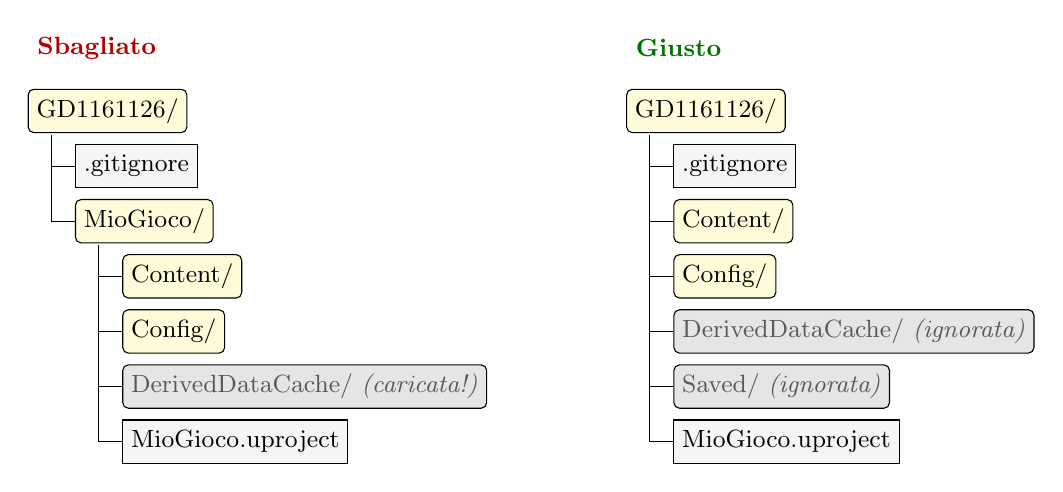
\begin{tikzpicture}[
  font=\small,
  gd13dir/.style={draw, rounded corners=2pt, fill=yellow!15, minimum
    height=0.55cm, inner sep=3pt, anchor=west},
  gd13file/.style={draw, fill=gray!8, minimum height=0.55cm, inner sep=3pt,
    anchor=west},
  gd13no/.style={draw, rounded corners=2pt, fill=gray!20, text=gray!70!black,
    minimum height=0.55cm, inner sep=3pt, anchor=west}]
  % sbagliato
  \node[font=\small\bfseries, text=red!70!black, anchor=west] at (0,0.8)
       {Sbagliato};
  \node[gd13dir] (r1) at (0,0) {GD1161126/};
  \node[gd13file] at (0.6,-0.7) {.gitignore};
  \node[gd13dir] (p1) at (0.6,-1.4) {MioGioco/};
  \node[gd13dir] at (1.2,-2.1) {Content/};
  \node[gd13dir] at (1.2,-2.8) {Config/};
  \node[gd13no] at (1.2,-3.5) {DerivedDataCache/ \emph{(caricata!)}};
  \node[gd13file] at (1.2,-4.2) {MioGioco.uproject};
  \draw (0.3,-0.3) |- (0.6,-0.7); \draw (0.3,-0.7) |- (0.6,-1.4);
  \draw (0.9,-1.7) |- (1.2,-2.1); \draw (0.9,-2.1) |- (1.2,-2.8);
  \draw (0.9,-2.8) |- (1.2,-3.5); \draw (0.9,-3.5) |- (1.2,-4.2);
  % giusto
  \begin{scope}[xshift=7.6cm]
  \node[font=\small\bfseries, text=green!45!black, anchor=west] at (0,0.8)
       {Giusto};
  \node[gd13dir] at (0,0) {GD1161126/};
  \node[gd13file] at (0.6,-0.7) {.gitignore};
  \node[gd13dir] at (0.6,-1.4) {Content/};
  \node[gd13dir] at (0.6,-2.1) {Config/};
  \node[gd13no] at (0.6,-2.8) {DerivedDataCache/ \emph{(ignorata)}};
  \node[gd13no] at (0.6,-3.5) {Saved/ \emph{(ignorata)}};
  \node[gd13file] at (0.6,-4.2) {MioGioco.uproject};
  \draw (0.3,-0.3) |- (0.6,-0.7); \draw (0.3,-0.7) |- (0.6,-1.4);
  \draw (0.3,-1.4) |- (0.6,-2.1); \draw (0.3,-2.1) |- (0.6,-2.8);
  \draw (0.3,-2.8) |- (0.6,-3.5); \draw (0.3,-3.5) |- (0.6,-4.2);
  \end{scope}
\end{tikzpicture}
\caption{Dove va il progetto. A sinistra la cartella del progetto è stata
trascinata intera dentro il repository: le regole del \texttt{.gitignore} non
la riconoscono più e le cache finiscono online. A destra è stato spostato il
\emph{contenuto}: \texttt{.gitignore}, cartelle di Unreal e \texttt{.uproject}
stanno allo stesso livello.}
\label{gd13:fig:cartelle}
\end{figure}

\paragraph{Aprire il progetto spostato.} Federica non sa più come aprire il
progetto condiviso: ``facilissimo, basta che vai sulla cartella e fai
\textbf{doppio clic} sul \texttt{.uproject}''. Quando si sposta un progetto
dalla sua cartella originale, infatti, l'\textbf{Epic Games Launcher} potrebbe
non mostrarlo più tra i progetti, ``perché non sa più dove cavolo è''. Se il
doppio clic non funziona (``l'Epic Games Launcher non ti ha associato i file''),
dal launcher si va su \textbf{I miei progetti}, poi \textbf{Sfoglia} in basso a
destra, e si seleziona la cartella del repository (di solito in
\texttt{Documenti/GitHub}). Se Unreal chiede di convertire il progetto, si
sceglie \textbf{More options $\rightarrow$ Skip conversion}: ``salta la
conversione e sei a posto''. Il docente sospetta che qualcuno abbia usato una
versione dell'engine diversa e abbia ``sovrascritto una roba''; ``non è un
problema''.

\paragraph{Mai versioni diverse.} ``Cosa super importante che non dovrei neanche
dire: non utilizzate versioni diverse di Unreal. Mi raccomando, perché sennò si
rompe tutto quanto nel giro di 25 secondi.'' Un progetto aperto con una
versione più nuova viene convertito e non torna indietro (lo stesso principio
visto per gli asset di Fab, sezione~\ref{gd12:sec:fab}).

% ---------------------------------------------------------------------
\section{Commit e push}
\label{gd13:sec:commit}

Spostato il progetto, GitHub Desktop se ne accorge da solo: nella scheda
\textbf{Changes}\footnote{Trascritto come ``Gengis''.}, sulla sinistra,
compaiono \textbf{tutti i cambiamenti} rispetto all'ultima versione online, in
questo caso tutto il progetto: il personaggio, il codice, i cubi, i cilindri,
eccetera.

\paragraph{Il commit.} ``Dobbiamo fare il nostro primo \textbf{commit}. I commit
sono dei cambiamenti che noi mandiamo al server, fondamentalmente.'' Ogni
commit deve avere un \textbf{titolo}, che di solito descrive \textbf{che cosa si
è cambiato}: ``ho integrato lo sparo'', ``ho creato il salto'', oppure, qui,
``progetto creato''. Poi si preme \textbf{Commit to main}.

\paragraph{Il push.} Il commit, da solo, resta sul proprio computer. Per
mandarlo davvero online bisogna premere \textbf{Push origin}, il pulsante in
alto. Ed ecco il consiglio pratico più importante della lezione:
\begin{quote}
Quando dovete fare qualsiasi cosa, se non sapete cosa fare, premete sempre qui
in alto, perché questo tasto permette di scaricare, caricare, controllare: fa
tutto qui. Un tasto solo, è sempre lì.
\end{quote}
È il pulsante di sincronizzazione in alto a destra, che cambia nome a seconda
della situazione: \emph{Publish repository} o \emph{Publish branch} la prima
volta, \emph{Fetch origin} per controllare se ci sono novità, \emph{Pull
origin} per scaricarle, \emph{Push origin} per caricare. Finito il push, la
lista dei cambiamenti è vuota: ``ora che non c'è più niente qua, siamo a
posto''. Aggiornando la pagina del repository sul sito si vedono i file caricati
(tabella~\ref{gd13:tab:gitignore}).

\paragraph{Una feature, un commit.} Chi lavora si dimentica facilmente di
caricare: in aula, alla prima prova, il docente controlla la history e ``no, non
vedo caricamenti''. Il motivo è sempre lo stesso: ``dovete fare commit
\emph{e poi} push qui in alto, se no non funziona''.

\paragraph{Approfondimento: scrivere bene i messaggi di commit.} Il titolo di un
commit è ciò che i compagni (e il docente) leggeranno nella history. La
convenzione più diffusa è quella suggerita implicitamente dagli esempi del
docente: una frase breve, al presente o al passato, che dica \emph{che cosa}
cambia per il gioco (``aggiunto il doppio salto'', ``corretta la collisione
della porta''), non ``modifiche'' o ``fix''. Un commit dovrebbe contenere un
solo cambiamento logico: così, se qualcosa si rompe, è facile capire quale
commit l'ha rotto e tornare indietro solo di quello.

% ---------------------------------------------------------------------
\section{I collaboratori}
\label{gd13:sec:collaboratori}

``Ora, quello che vorrei fare è chiaramente invitarvi tutti, in modo da poter
collaborare su questo progetto.'' Il docente chiede a ciascuno di mandare, nella
chat della classe su Discord, la \textbf{mail} usata per iscriversi a GitHub
oppure il \textbf{nome utente}. Dalle impostazioni del repository
(\emph{Settings $\rightarrow$ Collaborators $\rightarrow$ Add people}) li
aggiunge uno per uno.

\paragraph{Accettare l'invito.} Una volta invitati, arriva una \textbf{mail} con
la richiesta di conferma: ``dovete confermarlo e così ci siete''. Il docente
controlla: alcuni non hanno ancora accettato, ``quindi accettate in fretta''.
Se la mail non arriva, ``basta che vai lì e accetti'': l'invito si trova anche
sul sito.

\paragraph{Da ora, tutti sul progetto del docente.} Accettato l'invito, si clona
il repository del docente: \textbf{File $\rightarrow$ Clone repository}, e lo si
cerca nella lista (``magari fate un refresh e vi esce fuori''); se non compare,
si va nella scheda \textbf{URL} e si incolla il link che il docente ha mandato
in chat, ``una cosa che finisce con \texttt{.git}''. Il clone scarica tutto; con
Show in Explorer e doppio clic sul \texttt{.uproject} ``vi si apre il mio
progetto, non il vostro''. ``Da ora in poi non lavorerete più sul vostro,
lavorerete sul mio, tutti quanti.'' E una raccomandazione: ``per ora, sul
progetto non cambiate nulla, ok? Poi facciamo casini''.

A una domanda del docente, nessuno in classe conosceva GitHub prima di questa
lezione.

% ---------------------------------------------------------------------
\section{Fetch e pull, a engine chiuso}
\label{gd13:sec:pull}

\paragraph{Il primo scambio.} ``Ammettiamo che io stia lavorando su questo
progetto e voglia creare un nuovo Blueprint.'' Il docente crea un Blueprint
qualsiasi, lo chiama \textbf{Ciao} e salva. ``GitHub si accorge automaticamente
che Ciao è stato creato'': compare in Changes. Commit (``ho creato Ciao''),
push. Dall'altra parte, chi aveva già scaricato il progetto preme
\textbf{Fetch}; se ci sono novità compare il pulsante \textbf{Pull}, che le
scarica. Riaprendo il progetto, ``vi appare il Ciao, il bellissimo Blueprint
che c'è qua''. ``Questo è il principio proprio di base.''

\paragraph{Fetch e pull.} Le due operazioni sono diverse:
\begin{itemize}
  \item \textbf{Fetch} \emph{controlla} se online ci sono modifiche nuove, senza
        toccare i file locali. E non lo fa solo per il proprio branch: ``lui fa
        fetch di tutti i branch'' (i branch si vedranno nella
        sezione~\ref{gd13:sec:branch});
  \item \textbf{Pull} \emph{scarica} quelle modifiche e aggiorna i file sul
        disco.
\end{itemize}

\paragraph{La regola d'oro: engine chiuso quando si scarica.}
\begin{quote}
Mi raccomando, quando prendete qualcosa dovete sempre avere l'engine chiuso.
Quando caricate qualcosa potete lasciarlo aperto tranquillamente, ma quando
scaricate deve essere chiuso per forza.
\end{quote}
Il commit e il push si possono fare a engine aperto; il \textbf{pull} (``cioè
prendere le cose'') \textbf{no, assolutamente}. Lo stesso vale per il cambio di
branch (``lo switch di branch è sempre con l'engine chiuso'', si veda la
sezione~\ref{gd13:sec:branch}). Il docente lo ripete più volte durante la
lezione, anche a chi ha problemi: ``quando pullate, sempre l'engine chiuso. Mi
raccomando, se no non funziona niente''. Il motivo è che Unreal tiene in memoria
gli asset aperti e, al salvataggio, riscriverebbe sopra ai file appena scaricati
le proprie versioni vecchie.

\paragraph{La routine quotidiana.} Due abitudini da prendere subito:
\begin{itemize}
  \item \textbf{prima di aprire il progetto}, ogni volta che si torna a
        lavorare, si fa \textbf{fetch}, ``che non si sa mai'', e se ci sono
        novità \textbf{pull} (``tanto è un tasto solo, sempre questo''):
        altrimenti si lavora sulla versione vecchia;
  \item \textbf{quando si finisce di lavorare}, si fa sempre \textbf{push},
        ``perché altrimenti gli altri non possono vedere le vostre modifiche, e
        poi ci si vede il giorno dopo che tutti quanti hanno conflitti strani,
        perché non avete caricato voi, non hanno caricato loro, non avete preso
        le modifiche, eccetera. È avvenuto molto spesso, sfortunatamente.''
\end{itemize}

\begin{figure}[htbp]
\centering
\begin{tikzpicture}[
  font=\small, node distance=1.2cm and 2.4cm,
  gd13box/.style={draw, rounded corners=3pt, align=center, minimum width=3.2cm,
    minimum height=1.1cm, fill=#1},
  gd13arr/.style={-{Stealth[length=2.6mm]}, thick},
  gd13lab/.style={font=\footnotesize\bfseries, fill=white, inner sep=1.5pt}]
  \node[gd13box=blue!8] (wd) {\textbf{Cartella locale}\\\footnotesize i file
        su cui lavora Unreal};
  \node[gd13box=orange!12, right=of wd] (loc) {\textbf{Repository locale}\\
        \footnotesize i commit sul proprio PC};
  \node[gd13box=green!12, right=of loc] (rem) {\textbf{GitHub}\\
        \footnotesize il repository online};
  \draw[gd13arr] ([yshift=3mm]wd.east) -- node[gd13lab, above=1pt] {commit}
        ([yshift=3mm]loc.west);
  \draw[gd13arr] ([yshift=3mm]loc.east) -- node[gd13lab, above=1pt] {push}
        ([yshift=3mm]rem.west);
  \draw[gd13arr, dashed] ([yshift=-3mm]rem.west) -- node[gd13lab, below=1pt]
        {fetch} ([yshift=-3mm]loc.east);
  \draw[gd13arr] (rem.south) -- ++(0,-0.7) -| node[gd13lab, pos=0.25, below=2pt]
        {pull (= fetch + aggiornamento dei file) \quad\textcolor{red!70!black}{engine chiuso!}}
        (wd.south);
  \draw[gd13arr] (rem.north) -- ++(0,0.7) -| node[gd13lab, pos=0.25, above=2pt]
        {clone: la prima volta, scarica tutto} (wd.north);
\end{tikzpicture}
\caption{Le operazioni di base di Git, come le si usa da GitHub Desktop. Commit
e push si possono fare anche con l'engine aperto; pull e cambio di branch solo
a engine chiuso.}
\label{gd13:fig:operazioni}
\end{figure}

\paragraph{La history non dimentica nulla.} Accanto a Changes c'è la scheda
\textbf{History}, con tutti i cambiamenti fatti nel tempo. E qui un
avvertimento serio:
\begin{quote}
Mi raccomando, su GitHub non si può mai cancellare nulla. Nel senso: se voi
avete caricato le vostre password, per dire, le vostre foto imbarazzanti, è un
casino. Perché dalla storia non si cancella mai nulla. Bisogna ricreare tutto
quanto da zero.
\end{quote}
Quindi ``non caricate mai nulla che non volete caricare'', e fate ``super
attenzione, soprattutto se il repository è pubblico, perché tutti quanti possono
vedere tutto''.

\paragraph{Approfondimento: perché ``non si cancella''.} Ogni commit di Git
contiene un riferimento al commit precedente: la history è una catena in cui
ogni anello dipende da quelli prima. Cancellare un file con un nuovo commit lo
toglie dalla versione attuale, ma non dai commit vecchi, dove resta leggibile da
chiunque abbia accesso al repository. Toglierlo davvero significa
\emph{riscrivere} la history (con strumenti appositi) e chiedere a tutti di
riscaricarla; e se nel frattempo qualcuno ne aveva una copia, o il repository
era pubblico, il file va comunque considerato compromesso: una password
caricata per errore si cambia, non si nasconde.

\paragraph{Problemi di login.} Durante le prove Federica e un'altra studentessa
non riescono a fare push: ``c'è un problema di credenziali''. Il docente fa
provare il \textbf{logout e un nuovo login} (\emph{File $\rightarrow$ Options
$\rightarrow$ Accounts $\rightarrow$ Sign out}, poi \emph{Sign in} e
\emph{Continue with browser}); in un caso il login chiedeva di Electron, e il
docente sospetta un conflitto con un'installazione precedente. Alla fine si
scopre la causa: proprio in quel momento GitHub Desktop si stava
\textbf{aggiornando} (``c'è un update di GitHub proprio adesso''), e questo
dava problemi di login. ``Poteva anche segnalarlo meglio.''

% ---------------------------------------------------------------------
\section{I conflitti}
\label{gd13:sec:conflitti}

Per vedere che cosa succede quando due persone toccano la stessa cosa, il
docente chiede a tutti di modificare il Blueprint \emph{Ciao}: ``mettete
sull'Event Graph un Print String, quello che volete. Fate un cambiamento
qualsiasi su questo oggetto. Compila, salva. Poi chiudete l'engine e lo
caricate''. Lui stesso fa una modifica sullo stesso file \emph{prima} di
riscaricare quelle degli altri, ``vedrete che vi darà dei problemi''.

Ed ecco il risultato: ``si è rotto, perché chiaramente facendo dei cambiamenti
sia io che voi sullo stesso file senza prima scaricare i miei o i vostri, si
creano dei \textbf{conflitti}''. GitHub ``dice: guarda, io ho queste due
versioni qui, quale devo tenere, quale devo non tenere?''

\paragraph{Un file binario: o il mio o il tuo.} Un asset di Unreal (un
Blueprint, una mappa, un materiale) è un file \textbf{binario}, non un testo
riga per riga: Git non può fondere le due versioni. ``Non funziona che prenda
entrambe le modifiche. Se è su un file singolo, o prendo il tuo o prendo il mio,
non ci sono vie di mezzo.'' Una delle due versioni va persa.

\paragraph{La soluzione: lavorare su file diversi.} ``Quello che si fa per
evitare questi overlap, questi conflitti, è cercare di lavorare su branch
diversi'', e soprattutto fare in modo che ``due persone non lavorino sugli
stessi identici file, perché altrimenti è un problema''.

% ---------------------------------------------------------------------
\section{I branch e il merge}
\label{gd13:sec:branch}

\subsection{Come un albero}

``Proprio come un albero: c'è il branch, questo qui, \textbf{main}, che è quello
principale, è proprio il tronco. E poi si può diramare in rami diversi. I rami
poi si possono anche \textbf{ricongiungere}: questa è la parte importante.''

Il docente chiede a tutti di fare prima \textbf{fetch e pull} delle ultime
modifiche, e poi di crearsi \textbf{un branch a testa}: \textbf{New branch} (dal
menu dei branch in alto), un nome, ``magari il vostro nome'', e \textbf{Create
branch}. Poi \textbf{Publish branch}, per caricare il branch sul repository e
renderlo visibile agli altri. Nella lista compaiono via via ``Junior,
Francesca'' e gli altri. A Federica, che crea il suo più tardi, il docente
raccomanda di non usare caratteri speciali nel nome, ``perché sennò poi
impazzisce''.

\subsection{Le filosofie dei nomi}

``Ci sono filosofie diverse.''
\begin{itemize}
  \item Branch \textbf{per persona}: ognuno lavora sul suo.
  \item Branch \textbf{per feature}, cioè per singola modifica (``il doppio
        salto'', ``il nuovo menu'').
  \item Branch \textbf{per dipartimento} (programmazione, arte, level design).
  \item Branch di \textbf{release}, e poi vari branch di \textbf{alpha},
        \textbf{beta} e così via.
\end{itemize}
``Ci sono un sacco di tipi di nomi diversi. Voi dovete capire, quando entrate in
un progetto, che nomenclatura si usa.'' Il docente, di solito, sui progetti più
grandi lavora \textbf{per feature}, sui progetti piccoli \textbf{con i nomi
delle persone}. L'importante resta che due persone non lavorino sugli stessi
file.

\subsection{Passare da un branch all'altro}

``Come faccio a vedere i cambiamenti che sta facendo Francesca mentre io sono
qua? Semplicemente schiaccio qua e ora sono sul branch di Francesca.'' Da quel
momento, tutte le modifiche che si fanno e si caricano finiscono sul branch di
Francesca, non sul proprio; per tornare indietro si seleziona di nuovo il
proprio. Sempre a \textbf{engine chiuso}. E ``da un branch si può fare un altro
branch'': se, mentre si è sul proprio, si vuole provare una feature che parta da
lì, si crea un nuovo branch da quello corrente.

\paragraph{La prova.} ``Ora vi chiederei di andare a fare un po' di modifiche
sul progetto: lavorateci cinque minuti, fatemi una mini feature, quello che è,
non è importante.'' Il docente fa la sua: guardando un oggetto qualsiasi e
premendo \textbf{E}, l'oggetto viene \textbf{distrutto}, ``quindi posso far
scomparire tutto. Anche il terreno, chiaramente. Questa è la mia meccanica per
il mio gioco.'' Lorenzo, nel frattempo, crea una \textbf{cartella nuova} e la
carica: ``è apparsa a tutti quanti, perché lui ha pushato le sue modifiche''.
Qualsiasi file messo nella cartella del repository viene condiviso, se non è di
un tipo escluso dal \texttt{.gitignore}.

\subsection{Il merge}

Quando tutti hanno caricato le loro modifiche sui loro branch, il docente
mostra come \textbf{riunirle}.
\begin{enumerate}
  \item Si passa al branch \textbf{main} (a engine chiuso).
  \item \textbf{Fetch}, per controllare le novità, e \textbf{Pull}.
  \item Dal menu dei branch, \textbf{Choose a branch to merge into main}: si
        sceglie il branch da cui prendere le modifiche. ``Basta essere sul
        branch dove vogliamo portare le cose.''
  \item Se ci sono \textbf{conflitti}, GitHub Desktop li elenca file per file, e
        per ciascuno si sceglie quale versione tenere.
  \item Dopo ogni merge, \textbf{push}, ``perché così carica l'unione dei due
        branch''.
\end{enumerate}

\paragraph{I conflitti in pratica.} Il primo merge, con il branch del docente
stesso, dà subito un conflitto: lo stesso asset era stato modificato ``sia da me
quando ero qua, sia da me quando ero là''. Per Git sono come due persone
separate, e va scelta una versione: ``il mio di qua''. Il branch di Francesca:
nessun conflitto, perfetto. Quello di Antonino\footnote{Trascritto come ``Antonio''; nei capitoli precedenti lo studente compare come Antonino.}: ``fantastico''. Un altro
studente\footnote{Il nome è trascritto come ``Maracino''; non è possibile
ricostruirlo con certezza.} aveva lavorato sullo stesso file: nuovo conflitto,
e il docente sceglie la sua versione ``perché mi piace di più''. Stessa cosa per
gli ultimi branch: conflitto, scelta, push.

\paragraph{Il risultato.} Il progetto riaperto è ``l'unione di tutti quanti i
vostri progetti che avete fatto contemporaneamente''. La History mostra tutte le
storie combinate, con i nomi di tutti; nel livello c'è il \textbf{carro armato}
che ha fatto qualcuno, la trigger box riscalata, un Blueprint modificato
cancellando quello che c'era, e qualcuno ha anche messo il suo lavoro nella
mappa.

\begin{figure}[htbp]
\centering
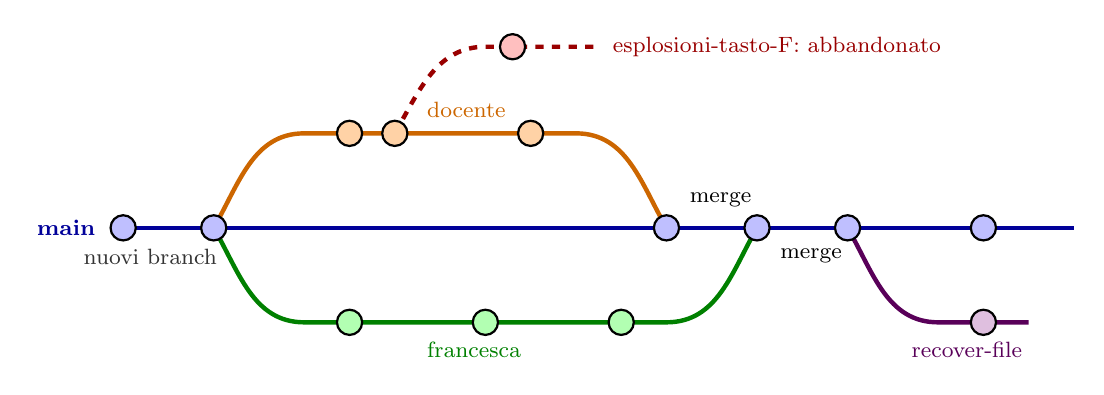
\begin{tikzpicture}[
  font=\small, x=1.15cm, y=1cm,
  gd13c/.style={circle, draw=black, thick, fill=#1, inner sep=0pt,
    minimum size=3.2mm},
  gd13br/.style={line width=1.6pt, draw=#1},
  gd13lbl/.style={font=\footnotesize, anchor=west}]
  % main
  \draw[gd13br=blue!60!black] (0,0) -- (10.5,0);
  \node[gd13lbl, text=blue!60!black, anchor=east] at (-0.2,0) {\textbf{main}};
  % branch docente
  \draw[gd13br=orange!80!black] (1,0) to[out=60, in=180] (2,1.2) -- (5,1.2)
       to[out=0, in=120] (6,0);
  \node[gd13lbl, text=orange!80!black] at (3.25,1.5) {docente};
  % branch Francesca
  \draw[gd13br=green!50!black] (1,0) to[out=-60, in=180] (2,-1.2) -- (6,-1.2)
       to[out=0, in=-120] (7,0);
  \node[gd13lbl, text=green!50!black] at (3.25,-1.55) {francesca};
  % branch abbandonato
  \draw[gd13br=red!60!black, dashed] (3,1.2) to[out=60, in=180] (4,2.3) -- (5.2,2.3);
  \node[gd13lbl, text=red!60!black] at (5.3,2.3) {esplosioni-tasto-F: abbandonato};
  % recover
  \draw[gd13br=violet!70!black] (8,0) to[out=-60, in=180] (9,-1.2) -- (10,-1.2);
  \node[gd13lbl, text=violet!70!black] at (8.6,-1.55) {recover-file};
  % commits
  \foreach \x in {0,1,6,7,8,9.5} \node[gd13c=blue!25] at (\x,0) {};
  \foreach \x in {2.5,3,4.5} \node[gd13c=orange!35] at (\x,1.2) {};
  \foreach \x in {2.5,4,5.5} \node[gd13c=green!30] at (\x,-1.2) {};
  \node[gd13c=red!25] at (4.3,2.3) {};
  \node[gd13c=violet!25] at (9.5,-1.2) {};
  \node[font=\footnotesize, anchor=west] at (6.15,0.35) {merge};
  \node[font=\footnotesize, anchor=west] at (7.15,-0.35) {merge};
  \node[font=\footnotesize, text=gray!40!black, anchor=north] at (0.3,-0.15) {nuovi branch};
\end{tikzpicture}
\caption{Il ``grafo'' dei branch, come lo mostrano i client più complessi.
Dal tronco (\emph{main}) partono i rami del docente e di Francesca, che poi
vengono riuniti con un merge; un ramo sperimentale viene abbandonato; dal
\emph{main} si crea più tardi un branch da un commit vecchio, per recuperare una
versione che funzionava (sezione~\ref{gd13:sec:tornare}).}
\label{gd13:fig:branch}
\end{figure}

% ---------------------------------------------------------------------
\section{Le mappe e la history}
\label{gd13:sec:mappe}

\paragraph{Le mappe si rompono per prime.} ``Le mappe sono una delle cose che
tendenzialmente si rompono più in fretta come conflitti, perché basta che uno
sposti una roba di un millimetro'' e la mappa intera diventa un file diverso:
``si può fare poco''. Unreal ha dei metodi per evitarlo, cioè dividere il mondo
in \textbf{sub-level}, livelli separati che poi si uniscono, ``però per gli open
world magari, non per robe piccole''. Per i progetti piccoli la regola è
organizzativa: anche chi lavora sul livello deve \textbf{coordinarsi} con gli
altri e non lavorarci nello stesso preciso momento.

\paragraph{Approfondimento: una mappa, tanti file.} I sub-level sono il sistema
classico (il \emph{level streaming}); per i mondi grandi Unreal 5 offre anche
il \emph{World Partition} con l'opzione \emph{One File Per Actor}, che salva
ogni oggetto del livello in un file separato: due persone che spostano oggetti
diversi toccano così file diversi, e i conflitti diventano rari. Per un progetto
d'aula basta però una regola semplice: chi tocca la mappa lo dice agli altri
prima di aprirla, e fa push appena ha finito.

\paragraph{Vedere le differenze in un Blueprint.} ``Altra cosa che però non vi
sto a spiegare troppo, perché sarebbe un pochettino lungo'': anche dentro Unreal
c'è un modo per vedere i \textbf{cambiamenti singoli su un Blueprint}, cioè come
è stato modificato tra un push e l'altro. ``Adesso non ci interessa; se però vi
dovesse servire, ditemelo e ve lo spiego.''\footnote{È lo strumento di
\emph{diff} dei Blueprint, che Unreal mette a disposizione quando il progetto è
collegato a un sistema di controllo di versione (\emph{Revision Control}):
mostra fianco a fianco due versioni dello stesso grafo, con i nodi aggiunti,
tolti o cambiati evidenziati. Tra i plugin dell'engine c'è infatti anche quello
per Git (sezione~\ref{gd13:sec:plugin}).}

\paragraph{La history come registro di chi ha lavorato.} Un avviso che riguarda
i voti:
\begin{quote}
Vi ricordo che sulla history si vede tutto, e chi cambia tutte le cose. Quindi
in un progetto di gruppo è possibile che io vada qua e che io guardi chi ha
fatto cosa, e se uno ha fatto tutto e l'altro non ha fatto niente, do un voto a
uno e all'altro no. Quindi io controllerò molto attentamente la history di
GitHub per capire i vari voti.
\end{quote}

% ---------------------------------------------------------------------
\section{Tornare indietro}
\label{gd13:sec:tornare}

\paragraph{Prima di caricare: Discard Changes.} ``Se fate delle modifiche e,
ancora prima di caricarle, vi accorgete che avete fatto un errore.'' Esempio: nel
livello del task il docente vuole vedere come sarebbe senza le
\textbf{monetine} (``diciamo che io le odio''), le cancella e salva; poi si
accorge che le voleva come prima. In GitHub Desktop, nella lista dei Changes:
\textbf{clic destro $\rightarrow$ Discard changes}, ``e torna come era prima''.
Le modifiche non sono state caricate: sono state \emph{scartate}.

\paragraph{Dopo: un branch da un commit vecchio.} Il caso classico: ``eh, ma io
l'ho provato tre settimane fa e funzionava. Non funziona più. E mo' che si
fa?'' Ci sono diversi metodi; il docente tende a fare così:
\begin{enumerate}
  \item si va nella \textbf{History} e si cerca un commit in cui si è sicuri
        che la cosa funzionasse (``io sono sicuro che qua, 39 minuti fa,
        funzionava'');
  \item \textbf{clic destro $\rightarrow$ Create branch from commit}, e lo si
        chiama per esempio \textbf{recover-file};
  \item quel branch è ``indietro nel tempo'': lo si apre, si controlla che cosa
        si era corrotto;
  \item poi si torna sul proprio branch attuale, ``e torno dove sono adesso''.
\end{enumerate}
Un branch creato e non ancora pubblicato non compare sul sito: ``non l'ho
pushato, quindi non appare su GitHub''.

\paragraph{I rami che muoiono.} I client più grafici, come Sourcetree,
disegnano tutto questo come un albero (figura~\ref{gd13:fig:branch}), ``ed è
probabile che ve lo faccia vedere qualcuno che usa quei programmi''. C'è il
branch principale, poi qualcuno lavora su un ramo, qualcun altro su un altro,
``poi si ricongiungono, oppure vanno a morire''. Esempio: ``come sarebbe il
nostro gioco se il personaggio, quando schiaccia la F, facesse delle esplosioni
gigantesche? È un'idea del cavolo, la provo su un branch, non funziona,
abbandono il branch. A posto, fine.''

\paragraph{Approfondimento: il branch come prototipo.} Questo uso dei branch è
la versione tecnica di due consigli che Jesse Schell, in \emph{The Art of Game
Design} (capitolo~8), dà sulla prototipazione: ogni prototipo deve
\textbf{rispondere a una domanda} (\emph{Prototyping Tip \#1}: ``sarebbe
divertente se, premendo F, ci fossero esplosioni gigantesche?''), e non bisogna
\textbf{affezionarsi} ai prototipi (\emph{Tip \#3}): se ne butteranno via molti,
e gli sviluppatori meno esperti ``fanno fatica a farlo, perché si sentono come
se avessero fallito''. Un branch costa pochi secondi, non sporca il lavoro degli
altri e, se l'idea non funziona, si abbandona; se funziona, un merge la porta nel
gioco. Il version control rende economico sbagliare, e quindi rende economico
sperimentare.

% ---------------------------------------------------------------------
\section{Il task, di nuovo, per chi era assente}
\label{gd13:sec:task}

Mentre gli altri provano Git, il docente chiede a Federica se abbia già una base
per il task: no, perché non ha ancora recuperato la lezione precedente. ``Hai
visto perlomeno la consegna? Allora guarda, la vediamo qua assieme.'' È lo
stesso task del capitolo~\ref{gd12:cap:array-timeline}
(sezione~\ref{gd12:sec:task}), riassunto così:
\begin{itemize}
  \item scadenza il \textbf{25}, ``quindi fondamentalmente fra una settimana e
        qualcosina'';
  \item un \textbf{platformer 3D}: si può partire tranquillamente dal
        \textbf{template 3D} di Unreal (in terza persona);
  \item almeno \textbf{tre livelli}, quindi tre mappe: quando si finisce una
        mappa si deve entrare nella successiva, con un \textbf{Open Level};
  \item il \textbf{personaggio base}, che cammina, salta, eccetera;
  \item degli \textbf{ostacoli}, che in alcuni casi possono far
        \textbf{ricominciare il livello}: trappole, buchi, ``qualcosa'' che può
        abbassare la vita oppure, ``se non vuoi complicarti troppo le cose'',
        semplicemente far ripartire il livello quando lo si tocca;
  \item delle \textbf{zone in cui il personaggio cambia} un pochettino: corre
        più in fretta, salta più in alto, ``o una roba di questo tipo'';
  \item \textbf{un livello con un timer}: se non lo si finisce entro il tempo,
        riparte, ``quindi finché non lo finisci abbastanza in fretta'';
  \item \textbf{Fab} per decorare un po' l'ambiente: ``non mi interessa che lo
        decori bene, basta che mi metti due asset da Fab. L'importante è il
        codice.''
\end{itemize}
Il consiglio a Federica è di creare subito il progetto, in \textbf{5.8} e con il
template in terza persona, per svilupparlo entro la volta successiva.

\paragraph{Le date.} Daniele chiede se questa sia l'ultima lezione prima della
consegna. No: ce n'è ancora una il \textbf{23} (il docente controlla il
calendario per sicurezza: ``sì, confermo''), e dal 23 restano altri due giorni
per lavorare. ``Tuttavia, se avete dei problemi, potete scrivermi prima.''

% ---------------------------------------------------------------------
\section{I plugin}
\label{gd13:sec:plugin}

\subsection{Mostrare i dati senza i widget}

Chiuso Git, si torna sul progetto della volta scorsa. Il docente vuole mostrare
``un po' di modi, intanto, per mostrare i dati del vostro gioco, perché per ora
ancora non conosciamo i \textbf{widget}, le interfacce visive''. Il primo metodo,
``che non è bellissimo, però vi amplia molto le possibilità'', sono i
\textbf{plugin}.

\paragraph{Edit $\rightarrow$ Plugins.} Unreal ha moltissimi plugin di base, e
tanti altri si scaricano da Fab. La lista completa si apre da \textbf{Edit
$\rightarrow$ Plugins}. Alcuni sono già \textbf{attivi} di base e funzionano,
altri no. ``Alcuni probabilmente non vi serviranno mai, la maggior parte, direi.
Alcuni possono essere utili.'' La finestra ha due sezioni principali:
\begin{itemize}
  \item \textbf{Built-in}: i plugin dell'engine base, ``già dentro l'engine:
        questi li attivi e funzionano già'';
  \item \textbf{Installed}: quelli scaricati (per esempio da Fab), ``che devi
        scaricare e poi ci sono''.
\end{itemize}
Con il pulsante \textbf{Add} si può anche creare un plugin proprio, ``non
approfondiamo per adesso''. Il docente invita a dare un'occhiata alla lista:
``alcuni possono tornarvi utili, però capisco che ce ne siano davvero tanti''.

\paragraph{Attivare un plugin.} Per esempio \textbf{Text 3D}, che permette di
\textbf{mettere dei testi nella scena}: ``se volete fare un timer, potete farlo
sfruttando questo plugin''. Si spunta, si conferma, e si \textbf{riavvia
l'engine}: ``tutte le volte che attivate o disattivate un plugin si deve
riavviare''. Dopo il riavvio, cercando \emph{text} nel pannello degli oggetti da
aggiungere si trova il nuovo attore, ``e ho questa funzionalità pazzesca di
mettere il testo nello scenario. Prima non potevo.''

\subsection{Un timer a schermo con il Text 3D}

``Dovessi fare un timer e non voglio ancora farlo vedere con un widget, perché
ancora non lo conosciamo'', si può usare il Text 3D come \textbf{componente}:
\begin{enumerate}
  \item si aggiunge un componente \textbf{Text 3D} al personaggio;
  \item lo si \textbf{attacca alla telecamera}, cioè lo si trascina sotto la
        \emph{Follow Camera} nella gerarchia dei componenti, ``così ora ce l'ho
        qui, fisso'', davanti alla visuale;
  \item da codice si usa \textbf{Set Text} e, come testo, il valore del timer.
\end{enumerate}
Il pin del testo è di tipo \emph{Text}, ma un float si può collegare
``tranquillamente'': Unreal inserisce da solo il nodo di \textbf{conversione}.
``Ci metto qualsiasi cosa qua, e uscirà dall'altra parte.'' Alla prova, il
testo compare a schermo con il valore dato. ``Non bellissimo'', ma funziona.

\subsection{Domande sui plugin}

\paragraph{Dove stanno.} Uno studente chiede dove finiscono i plugin scaricati.
``Di base, le cartelle sono due'':
\begin{itemize}
  \item una cartella \texttt{Plugins} \textbf{nel progetto}, che si può creare
        accanto a \texttt{Content}: i plugin messi lì valgono solo per quel
        progetto (e viaggiano con il progetto, anche su Git);
  \item una cartella \texttt{Plugins} \textbf{nell'engine}, cioè dove è stato
        installato Unreal: quelli di Fab, di solito, finiscono lì e poi si
        attivano progetto per progetto.
\end{itemize}
``In realtà, dalla 5.7, mi sembra, puoi anche mettere altre cartelle che vuoi
tu.'' I plugin \emph{Built-in} sono tutti nella cartella dell'engine,
``chiaramente, perché sono già qui''.

\paragraph{Perché non sono tutti attivi.} ``Perché molte feature potrebbero non
servirci'': quelle per la \textbf{realtà aumentata}, se il gioco non ce l'ha,
sarebbero ``soltanto un appesantimento''. Anzi, ``di base sono attivi anche
troppi, secondo me'', come l'\textbf{Apple Movie Player}: ``non penso che mi
serva''. Tutto ciò che è marcato \textbf{Chaos} riguarda invece la
\textbf{fisica} di Unreal.

\paragraph{Non disattivateli tutti.} ``Fate attenzione a non staccarli tutti,
perché, a parte che l'engine non si apre più, non c'è neanche più la finestra
dei plugin per riattivarli. Quindi è un casino: è proprio distruttivo.'' E un
aneddoto: ``l'ho visto fare'', da \emph{junior}: ti danno il progetto e ti dicono
``nel tempo libero disattiva tutti i plugin che puoi''. Stacchi, provi tutto il
gioco, funziona; stacchi ancora; ``e continui così, staccando più plugin che puoi
prima che si rompa il gioco. Lavoro molto divertente.'' (Lo scopo è alleggerire
la build finale.)

\paragraph{Qualche curiosità.} Scorrendo la lista il docente segnala: un plugin
per lavorare con \textbf{coordinate geografiche vere}, ``molto
interessante''\footnote{Probabilmente il plugin di \emph{georeferencing}
dell'engine; la trascrizione non riporta il nome.}; un plugin per
\textbf{Git}, ``perché si può collegare con Git'' direttamente da Unreal; i
plugin per i \textbf{capelli} (il sistema \emph{Groom}).

\paragraph{Approfondimento: il file .uplugin e il progetto.} L'elenco dei plugin
attivi in un progetto è salvato nel file \texttt{.uproject}, che è un semplice
file di testo: attivare un plugin \emph{built-in} cambia solo quel file, e su Git
basta condividerlo perché tutti abbiano lo stesso plugin attivo. Un plugin messo
nella cartella dell'engine, invece, non viaggia con il progetto: se un compagno
non l'ha installato, il progetto non si apre o perde delle funzioni. Per un
lavoro di gruppo conviene quindi mettere i plugin scaricati nella cartella
\texttt{Plugins} \emph{del progetto}, attenti al limite dei 100~MB
(sezione~\ref{gd13:sec:limiti}).

% ---------------------------------------------------------------------
\section{Il vecchio input system}
\label{gd13:sec:input}

\subsection{Due sistemi}

``Allora, di input system, in realtà, ce ne sono due. C'è quello vecchio e c'è
quello nuovo. Noi purtroppo vedremo quello vecchio, perché quello nuovo è un
casino, quindi lo vedremo più avanti.'' Il nuovo (l'\textbf{Enhanced Input}) è
quello che il template in terza persona usa già: sono gli oggetti di input che
si vedono nella cartella del template. ``Si possono utilizzare, chiaramente, ve
li spiegherò, ma più avanti, perché ora sono un po' troppo complessi.'' Il
docente aggiunge che, concettualmente, quelli vecchi ``sono molto più
intuitivi''.

\paragraph{Dove si trovano.} In \textbf{Edit $\rightarrow$ Project Settings},
categoria \textbf{Input}. L'editor avvisa che sono \textbf{deprecati}, ``perché
non sono più quelli nuovi, insomma''. ``Tuttavia penso che li manterranno ancora
per un bel po'.''

\subsection{Action Mappings e Axis Mappings}

Sono di due tipi:
\begin{itemize}
  \item gli \textbf{Action Mappings} sono \textbf{i tasti}, ``quindi sì o no'':
        sto premendo il tasto F, sì oppure no;
  \item gli \textbf{Axis Mappings} sono per i \textbf{valori con la virgola}:
        ``per esempio ho un controller, lo sto muovendo magari in avanti di
        0,5'', e il gioco deve registrare questa differenza.
\end{itemize}

\paragraph{Un'azione: Fire.} Con il \textbf{+} accanto ad Action Mappings si crea
una nuova azione. ``Quando ho il mio personaggio, premo il tasto sinistro del
mouse, spara'': la si chiama \textbf{Fire} e le si assegna un tasto. Nel menu ci
sono ``tutti quanti i tasti possibili, tutte le console possibili''. Se non si
vuole cercare, si preme l'icona della tastiera e poi \textbf{il tasto che si
vuole}: ``appare qua. Quindi facile.'' A una stessa azione si possono associare
\textbf{più tasti}, per esempio il tasto del mouse e il tasto X del controller:
``questo è compatibile con tutti quanti i vari dispositivi''.

\paragraph{Un asse: MoveUp.} Negli Axis Mappings si crea, per esempio,
\textbf{MoveUp}: \textbf{W} con scala \textbf{1}, per andare avanti, e
\textbf{S} con scala \textbf{$-1$}, per andare indietro, ``così ho un valore''.
Con un controller, lo stesso asse restituisce valori intermedi ``in base a quanto
muovo il joystick''. Vale anche per il \textbf{VR}.

\begin{table}[htbp]
\centering
\small
\begin{tabular}{p{2.6cm}p{5cm}p{5.4cm}}
\toprule
 & \textbf{Action Mapping} & \textbf{Axis Mapping}\\
\midrule
Valore & premuto / non premuto (sì o no) & un numero con la virgola, anche
negativo\\
Esempio a lezione & \emph{Fire}: tasto sinistro del mouse, tasto X del
controller & \emph{MoveUp}: W $= 1$, S $= -1$, stick del controller
($0{,}5$, \dots)\\
Evento nel Blueprint & \emph{InputAction Fire}, con le uscite
\emph{Pressed} e \emph{Released} & \emph{InputAxis MoveUp}, chiamato a ogni
frame con \emph{Axis Value}\\
Usi tipici & saltare, sparare, interagire, aprire il menu & camminare, guidare,
mirare, ruotare la telecamera\\
\bottomrule
\end{tabular}
\caption{I due tipi di mappatura del vecchio input system (\emph{Project
Settings $\rightarrow$ Input}).}
\label{gd13:tab:input}
\end{table}

\subsection{Usarli nel Blueprint}

Nel Blueprint del personaggio si cerca il nome dell'azione, \emph{Fire}, e si
trova l'\textbf{evento} corrispondente, ``che ho scritto dall'altra parte''.
Collegato a un Print String con il testo ``A'', basta premere Play e cliccare:
``vedete che viene fuori il testo, perché effettivamente è lì. Quindi prende
l'input del tasto che gli ho assegnato.''

\begin{figure}[htbp]
\centering
\begin{bpgraph}
  \bpnode[2]{fi}{0,0}{bpHEvent}{InputAction Fire\\\bpsub{Action Mapping}}{3.2}{}{exec/Pressed, exec/Released, struct/Key}
  \bpnode{ps}{4.6,0}{bpHFunc}{Print String}{3.0}{exec/, str/In String \bpval{A}}{exec/}
  \bpnode[2]{ax}{0,-2.6}{bpHEvent}{InputAxis MoveUp\\\bpsub{Axis Mapping}}{3.2}{}{exec/, float/Axis Value}
  \bpnode{ps2}{4.6,-2.6}{bpHFunc}{Print String}{3.0}{exec/, str/In String}{exec/}
  \bpwire{exec}{fi-o1}{ps-i1}
  \bpwire{exec}{ax-o1}{ps2-i1}
  \bpwire{float}{ax-o2}{ps2-i2}
  \bpnote{8.0,-2.6}{W $\rightarrow$ 1\\S $\rightarrow$ $-1$\\nulla $\rightarrow$ 0}
\end{bpgraph}
\caption{Gli eventi generati dalle mappature: l'azione \emph{Fire} ha
un'uscita quando il tasto viene premuto e una quando viene rilasciato; l'asse
\emph{MoveUp} viene chiamato continuamente e porta con sé il valore. (Il
collegamento di un float al Print String inserisce da solo la conversione in
stringa.)}
\label{gd13:fig:input}
\end{figure}

\paragraph{Approfondimento: Action e Axis secondo Romero e Sewell.} Il libro di
Romero e Sewell (capitolo~6) usa proprio questo sistema per aggiungere al
personaggio uno \emph{sprint} e uno \emph{zoom}: due Action Mappings
(\emph{Sprint} su Shift sinistro, \emph{Zoom} sul tasto destro del mouse),
``perché sono azioni semplici, o attive o inattive''. Gli autori riassumono la
differenza con le stesse parole del docente: le Action Mappings sono eventi di
pressione di un tasto o di un clic; le Axis Mappings associano movimenti ed
eventi che hanno un \emph{intervallo} di valori, come W e S che agiscono sulla
stessa azione di movimento ``ma ai due estremi dell'intervallo''.

% ---------------------------------------------------------------------
\section{I componenti}
\label{gd13:sec:componenti}

\subsection{Che cos'è un componente}

``Ora mi piacerebbe approfondire un minimo i \textbf{componenti}.'' In Unreal se
ne sono già visti tanti: il \emph{Text 3D} appena aggiunto è un componente,
la \emph{Follow Camera} è un componente, la \emph{mesh} del personaggio è un
componente: ``è pieno di componenti''. Non solo nel personaggio: in tutti i
Blueprint. E si possono \textbf{creare}.

\paragraph{Perché crearne uno.} Esempio: il \textbf{sistema di vita}. ``Non lo
creiamo dentro il personaggio, perché altrimenti poi, se devo metterlo sui
nemici, devo metterlo sulle scatole che quando le picchi si distruggono, eccetera,
dovrei ricopiarlo un milione di volte in tutti i vari sistemi.'' Un componente
si scrive una volta e si aggiunge a chi serve. ``E poi magari vogliamo proprio
delle feature che siano legate allo spazio, a dove si trovano.''

\subsection{Actor Component e Scene Component}

Si crea con \textbf{clic destro $\rightarrow$ Blueprint Class}, ma questa volta,
``a differenza di tutte le altre volte'', non un Actor: un
\textbf{componente}. I componenti si dividono in due categorie, ``molto
facili'':
\begin{itemize}
  \item l'\textbf{Actor Component} non ha uno spazio, ``non è in una posizione
        precisa'': il sistema della vita ``non ha una posizione, è lì,
        semplicemente sull'oggetto'';
  \item lo \textbf{Scene Component} ha una posizione (una \emph{transform}):
        una mesh, il punto da cui parte un suono, la barra della vita sopra la
        testa di un nemico, ``e tutte queste altre funzionalità''.
\end{itemize}

\begin{table}[htbp]
\centering
\small
\begin{tabular}{p{2.8cm}p{5cm}p{5.2cm}}
\toprule
 & \textbf{Actor Component} & \textbf{Scene Component}\\
\midrule
Posizione nel mondo & nessuna & sì: location, rotation, scale\\
Si può attaccare ad altri componenti & no & sì, come figlio di un altro
Scene Component\\
Esempi & vita, stamina, inventario, punteggio, esperienza & mesh, telecamera,
sorgente di un suono, barra della vita sopra la testa, cerniera di una porta\\
\bottomrule
\end{tabular}
\caption{Le due famiglie di componenti. Gli Scene Component erano già comparsi
come ``cerniere'' della doppia porta nel capitolo~\ref{gd12:cap:array-timeline}.}
\label{gd13:tab:componenti}
\end{table}

\subsection{L'Health Component}

Per la vita basta un \textbf{Actor Component}, che il docente chiama
\textbf{HealthComponent}. ``Ve lo spiego più che altro perché non è troppo
difficile concettualmente, e capendo questo capite anche come funzionano gli
altri componenti, già creati di base dall'engine o dal programmatore.''
Aprendolo, ``come vedete è super familiare'': c'è il \emph{Begin Play}, ci sono
le stesse cose già viste.

\paragraph{La variabile.} Si crea una variabile \textbf{CurrentHealth}, la vita
attuale, di tipo \textbf{float} (``numeri con la virgola''), con valore di
partenza \textbf{100}, ``che mi sembra un buon numero di vita iniziale''. Per
ora ``è semplicemente un numerino'', ma può tornare molto utile.

\paragraph{Aggiungerlo al personaggio.} Nel \textbf{BP\_ThirdPersonCharacter},
\textbf{Add} nel pannello dei componenti, si cerca \emph{health} e si trova
l'\textbf{HealthComponent}, ``quello che ho appena creato''. Si aggiunge, e
selezionandolo si vede la sua vita nel pannello \emph{Details}.

\paragraph{Un valore diverso per ogni personaggio.} Il vantaggio è immediato:
``se ho cinque personaggi, basta che li apro e modifico qua la loro vita: uno ce
ne avrà 100, uno 150, l'altro 20''. Per i vari tipi di nemici si modifica
tranquillamente da lì. Lo scopo dei componenti è ``tagliare'' il codice, cioè
non accumulare tutto nell'Event Graph del personaggio, ``soprattutto per
funzionalità che sono in condivisione tra diversi personaggi''.

\paragraph{Leggere e scrivere la vita.} Si accede ai dati del componente come
si è sempre fatto con il \emph{Character Movement}: si trascina il componente
nel grafo e si tira fuori \textbf{Get CurrentHealth} o \textbf{Set
CurrentHealth}. ``Stesso principio.''

\subsection{La Damage Area}

``Se ad esempio noi vogliamo fare un'area che ci fa danno, sfruttando le lezioni
precedenti'':
\begin{enumerate}
  \item un nuovo \textbf{Blueprint Class $\rightarrow$ Actor}, chiamato
        \textbf{DamageArea};
  \item dentro, \textbf{Add $\rightarrow$ Box Collision}, ``come abbiamo sempre
        fatto'';
  \item dal pannello dei dettagli della box, in fondo, l'evento
        \textbf{On Component Begin Overlap};
  \item un \textbf{Cast To BP\_ThirdPersonCharacter}, per controllare che sia
        il personaggio a entrare nella box;
  \item dal personaggio, però, la vita non si raggiunge direttamente, ``perché
        la vita non è sul personaggio puro, è sul componente'': si prende
        \textbf{Get HealthComponent};
  \item da lì, \textbf{Set CurrentHealth} con il valore \textbf{Get
        CurrentHealth $-$ 20}.
\end{enumerate}
``In realtà questa cosa qua la stiamo facendo dal giorno 1 con il character
speed'' (la velocità del personaggio, letta dal Character Movement nel
capitolo~\ref{gd7:cap:blueprint}): stessa roba.

\begin{figure}[htbp]
\centering
\resizebox{\linewidth}{!}{%
\begin{bpgraph}
  \bpnode[2]{ov}{0,0}{bpHEvent}{On Component Begin Overlap (Box)}{4.4}{}{exec/, obj/Other Actor}
  \bpnode{ca}{5.4,0}{bpHCast}{Cast To BP\_ThirdPersonCharacter}{4.6}{exec/, obj/Object}{exec/, exec/Cast Failed, obj/As BP Third Person Character}
  \bpnode{hc}{5.6,-3.1}{bpHPure}{Get HealthComponent}{3.4}{obj/Target}{obj/Health Component}
  \bpnode{gh}{9.6,-3.1}{bpHPure}{Get CurrentHealth}{3.0}{obj/Target}{float/}
  \bpnode{sub}{13.0,-2.4}{compact}{$-$}{1.4}{float/, float/\bpval{20}}{float/}
  \bpnode{set}{14.9,0}{bpHFunc}{Set CurrentHealth}{3.2}{exec/, obj/Target, float/Current Health}{exec/}
  \bpwire{exec}{ov-o1}{ca-i1}
  \bpwire{obj}{ov-o2}{ca-i2}
  \bpwire{exec}{ca-o1}{set-i1}
  \bpwire{obj}{ca-o3}{hc-i1}
  \bpwire{obj}{hc-o1}{gh-i1}
  \bpwire{obj}{hc-o1}{set-i2}
  \bpwire{float}{gh-o1}{sub-i1}
  \bpwire{float}{sub-o1}{set-i3}
\end{bpgraph}}
\caption{La prima versione della Damage Area: chi entra nella box viene
controllato con un cast; se è il personaggio, si prende il suo Health Component
e gli si tolgono 20 punti vita. ``Tecnicamente funziona'', ma non è il modo
migliore.}
\label{gd13:fig:damage-v1}
\end{figure}

\paragraph{La prova.} Per vedere che cosa succede, nel personaggio si stampa la
vita a ogni frame con un \textbf{Print String} (``quello che c'è nell'Health
Component, essendo il componente esposto, lo posso usare anche da qui''). Al
Play compare \textbf{100}; messa la Damage Area nel livello e camminandoci
dentro, ``vedete che mi scende. Quindi il codice sta funzionando
correttamente''.

\paragraph{Le reference.} Questo modo di raggiungere un componente si basa su un
concetto generale: ``questa cosa qua si chiama \textbf{reference}. Se ho la
reference a un oggetto qualsiasi, posso interagirci sempre.'' Ci sono anche le
\textbf{variabili private}, che non si possono toccare dall'esterno, ``ma non
lo facciamo adesso''. Una studentessa non trova più dove si aggiunge il
componente: ``lo trovi qua, tra tutti quanti gli altri componenti: lo cerchi e
ti esce''.

\subsection{Perché non basta}

``Funziona correttamente, però non è comodissimo. Soprattutto, diventa
complicato gestirlo così.'' Se tante cose fanno danno, e quando si subisce danno
devono succedere tante cose (la barra deve scendere, c'è il
\textbf{knockback}, c'è l'effetto visivo, il suono), ``chiaramente, se metto
tutta questa roba qua su ogni roba che mi fa danno, impazzisco''. Serve un modo
per scrivere il ``prendere danno'' \textbf{una volta sola}: le funzioni.

\paragraph{Approfondimento: Get Owner.} Romero e Sewell (capitolo~18) mostrano
anche il percorso inverso: dentro un componente, il nodo \textbf{Get Owner}
restituisce l'Actor che lo sta usando. È così che un Health Component può, per
esempio, distruggere il proprio proprietario quando la vita finisce, o leggere
la sua posizione per far partire un effetto, senza sapere in anticipo se è
attaccato al giocatore, a un nemico o a una cassa. Il libro costruisce un Actor
Component per l'esperienza e i livelli (\emph{BP\_ExpLevelComp}) e uno Scene
Component che fa ruotare uno scudo attorno al personaggio
(\emph{BP\_CircularMovComp}): gli stessi due casi, ``senza posizione'' e ``con
posizione'', della tabella~\ref{gd13:tab:componenti}.

% ---------------------------------------------------------------------
\section{Le funzioni}
\label{gd13:sec:funzioni}

\subsection{Un nodo fatto di nodi}

``Questa cosa c'è sia nei componenti, ma c'è anche nel Blueprint classico.
Anzi, vi consiglio di utilizzarla molto: le \textbf{funzioni}.'' Si creano dal
pannello \emph{My Blueprint}, con il \textbf{+} accanto a \emph{Functions}. Le
funzioni ``sono dei piccoli Blueprint, in realtà, dei piccoli nodi''.

\paragraph{La funzione Damage.} Nell'Health Component il docente crea una
funzione \textbf{Damage}, che farà danno al personaggio. L'idea è che il danno
non sia ``sottraiamo la vita e siamo a posto così'': in un punto unico si possono
aggiornare la barra della vita, gli effetti, il rumore, ``di conseguenza a
quanta vita ha, senza controllarla tutti i frame''.
\begin{enumerate}
  \item Dentro la funzione: \textbf{CurrentHealth $=$ CurrentHealth $-$
        \dots}, ma il \emph{quanto} non lo si scrive lì.
  \item Si aggiunge un \textbf{input}: selezionando la funzione, nel pannello
        \emph{Details}, \textbf{Inputs $\rightarrow$ +}, un parametro
        \textbf{DamageValue} di tipo \textbf{float}: ``come informazione di
        input a questa funzione, quanto danno deve prendere''.
  \item Il pin \emph{DamageValue} compare sul nodo d'ingresso della funzione, e
        lo si collega alla sottrazione.
\end{enumerate}
``Facendo questa piccolissima operazione, quello che abbiamo fatto è stato
\textbf{creare un nodo}.'' La funzione si trascina nel grafo e diventa un nodo
come gli altri: ``i nodi non sono soltanto prefatti, ma composti da altri nodi,
in alcuni casi''.

\paragraph{La Damage Area, versione due.} Nella Damage Area, al posto della
catena Get--sottrazione--Set, ``che è un po' bruttina'', si chiama
direttamente \textbf{Damage} con valore \textbf{20}. ``E così funziona molto
meglio, tra virgolette: se poi ci devo mettere dopo tante cose, funzioneranno
sempre, per qualsiasi sorgente di danno.''

\begin{figure}[htbp]
\centering
\begin{bpgraph}
  \bpnode{ca}{0,0}{bpHCast}{Cast To BP\_ThirdPersonCharacter}{4.6}{exec/, obj/Object}{exec/, exec/Cast Failed, obj/As BP Third Person Character}
  \bpnode{hc}{0.4,-3.1}{bpHPure}{Get HealthComponent}{3.4}{obj/Target}{obj/Health Component}
  \bpnode[2]{dm}{6.0,0}{bpHFunc}{Damage\\\bpsub{Target is Health Component}}{3.6}{exec/, obj/Target, float/Damage Value \bpval{20}}{exec/, float/Remaining Health}
  \bpwire{exec}{ca-o1}{dm-i1}
  \bpwire{obj}{ca-o3}{hc-i1}
  \bpwire{obj}{hc-o1}{dm-i2}
  \bpnote{6.0,-2.6}{tutto il resto (suono, morte,\\barra della vita\dots) sta\\dentro la funzione}
\end{bpgraph}
\caption{La Damage Area dopo l'introduzione della funzione: un solo nodo,
\emph{Damage}, con il valore del danno come input. Qualsiasi altra sorgente di
danno (lava, proiettili, nemici) userà lo stesso nodo.}
\label{gd13:fig:damage-v2}
\end{figure}

\subsection{Più input, un solo punto}

``Basta che vai qua e gli aggiungi: sugli input puoi mettere \emph{più}, e così
entra qui dentro.'' Una funzione può avere \textbf{più input} (e più output):
oltre al \emph{DamageValue}, per esempio, una \textbf{KnockbackForce}, poi
l'\textbf{Instigator}, ``che è chi mi ha fatto danno'', poi se applica qualche
\textbf{status}. ``Posso mettere tutto quanto qui dentro e funzionerà
correttamente.''

\paragraph{La morte, in un posto solo.} ``La cosa comoda è che, essendo un punto
unico dove noi aggiorniamo la vita, possiamo anche controllare molto facilmente
se il personaggio è morto oppure no.'' Dopo la sottrazione:
\textbf{CurrentHealth $\leq 0$} $\rightarrow$ \textbf{Branch} $\rightarrow$ se
vero, \textbf{Get Current Level Name} e \textbf{Open Level (by Name)}: ``in
questo modo mi assicura che appena finita la vita mi riparte il livello''
(lo stesso schema del capitolo~\ref{gd12:cap:array-timeline},
sezione~\ref{gd12:sec:ricarica}). E se si vuole un suono quando si prende danno,
basta un \textbf{Play Sound 2D} con il suono dentro, ``ovviamente''.

\subsection{Gli output e le funzioni pure}

\paragraph{Gli output.} Le funzioni ``possono avere anche altre due cosucce che
ovviamente tornano utili''. La prima: gli \textbf{output}. ``Posso avere delle
funzioni che hanno roba che entra e roba che esce.'' Per la funzione Damage,
per esempio, ``è morto sì o no'', oppure quanta vita rimane: con \textbf{Outputs
$\rightarrow$ +} compare un nodo \textbf{Return}, a cui si collega
\emph{CurrentHealth}, ``e quindi mi esce di qui''. ``Quindi può entrare roba,
può uscire roba, può solamente entrare o solamente uscire. Tutto quello che
volete.''

\paragraph{Le funzioni pure.} La seconda: spuntando \textbf{Pure} nei dettagli,
la funzione ``non vi chiede più i nodi bianchi, quelli di input e di output'',
cioè i pin di \textbf{esecuzione}: diventa un nodo che dà solo un valore. È la
differenza che si vede già tra i nodi dell'engine: un \emph{Get} o una
sottrazione sono puri, un \emph{Set Actor Location} ``non è puro, e infatti ha i
nodi che escono e che entrano''.

\begin{figure}[htbp]
\centering
\resizebox{\linewidth}{!}{%
\begin{bpgraph}
  \bpnode{en}{0,0}{bpHFunc}{Damage}{2.6}{}{exec/, float/Damage Value}
  \bpget{gh}{0.2,-2.5}{float}{Current Health}{2.2}
  \bpnode{sub}{3.4,-1.7}{compact}{$-$}{1.3}{float/, float/}{float/}
  \bpnode[1]{set}{5.2,0}{bpHVar}{SET}{2.2}{exec/, float/Current Health}{exec/, float/}
  \bpnode{le}{7.8,-1.9}{compact}{$\leq$}{1.5}{float/, float/\bpval{0}}{bool/}
  \bpnode{br}{9.8,0}{bpHFlow}{Branch}{2.1}{exec/, bool/Condition}{exec/True, exec/False}
  \bpnode{ps}{12.6,0}{bpHFunc}{Play Sound 2D}{2.6}{exec/, obj/Sound}{exec/}
  \bpnode{ol}{12.6,-1.8}{bpHFunc}{Open Level (by Name)}{3.4}{exec/, name/Level Name}{exec/}
  \bpnode{gl}{9.0,-3.6}{bpHPure}{Get Current Level Name}{3.6}{}{str/}
  \bpnode{rt}{16.6,0}{bpHFunc}{Return Node}{2.8}{exec/, float/Remaining Health}{}
  \bpwire{exec}{en-o1}{set-i1}
  \bpwire{float}{gh-o1}{sub-i1}
  \bpwire{float}{en-o2}{sub-i2}
  \bpwire{float}{sub-o1}{set-i2}
  \bpwire{exec}{set-o1}{br-i1}
  \bpwire{float}{set-o2}{le-i1}
  \bpwire{bool}{le-o1}{br-i2}
  \bpwire{exec}{br-o1}{ol-i1}
  \bpwire{exec}{br-o2}{ps-i1}
  \bpwire{str}{gl-o1}{ol-i2}
  \bpwire{exec}{ps-o1}{rt-i1}
  \bpwire{float}{set-o2}{rt-i2}
\end{bpgraph}}
\caption{L'interno della funzione \emph{Damage} nell'Health Component: un input
(\emph{Damage Value}), la sottrazione, il controllo della morte con il
ricaricamento del livello, il suono del colpo e un output con la vita rimasta.
Qualsiasi effetto futuro (knockback, barra, status) si aggiunge qui, una volta
sola.}
\label{gd13:fig:damage-funzione}
\end{figure}

Alla prova, camminando più volte nella Damage Area: ``tac, mi è ripartito il
livello, perché sono morto, come immaginavo''.

\subsection{Il limite: niente tempo}

``L'unica cosa scomoda delle funzioni è che non potete mettere cose che cambiano
nel tempo'': i \textbf{Delay} non si possono mettere, le \textbf{timeline} non
si possono mettere, ``vi dice proprio no''. Una funzione deve iniziare e finire
nello stesso istante. Lo ribadisce più avanti, rispondendo a Federica
(sezione~\ref{gd13:sec:colloquio}): si può anche tenere tutto il codice
nell'Event Graph principale, ``però è comodo renderlo in funzioni. L'unica cosa
veramente scomoda delle funzioni è che non possono esserci cose come i delay, i
wait, eccetera. Quindi per alcune cose è un pochettino scomodo; il resto si può
fare tranquillamente.''

\subsection{Collapse to Function}

``Se avete fatto qualcosa, tipo questo codice qua, e vi rendete conto che
funzionerebbe molto meglio come funzione, o non volete che stia qui in mezzo'':
si selezionano i nodi, \textbf{clic destro $\rightarrow$ Collapse to Function},
e Unreal crea una funzione con dentro quel codice, sostituendolo con il nodo.
``Super comodo.''

\paragraph{Usatele.} Le funzioni possono stare sia nei componenti sia nei
Blueprint classici, ``non c'è nessuna limitazione''. ``In teoria le funzioni
dovrebbero essere utilizzate veramente tanto, perché migliorano veramente molto
la leggibilità del codice, quanto può essere strutturato bene. C'è gente che fa
tutto con le funzioni.''

\begin{table}[htbp]
\centering
\small
\begin{tabular}{p{3.6cm}p{4.4cm}p{4.8cm}}
\toprule
 & \textbf{Funzione} & \textbf{Event Graph (eventi)}\\
\midrule
Input e output & sì, quanti se ne vuole & solo input (parametri
dell'evento personalizzato)\\
Delay, timeline, nodi latenti & no & sì\\
Chiamabile da altri Blueprint & sì, con una reference & sì (eventi
personalizzati)\\
Versione ``pura'' & sì, senza pin di esecuzione & no\\
Quando usarla & calcoli, azioni istantanee, logica riusata (il danno) &
sequenze nel tempo (il timer, la porta)\\
\bottomrule
\end{tabular}
\caption{Funzioni ed eventi a confronto, secondo quanto detto a lezione e le
regole dell'editor.}
\label{gd13:tab:funzioni}
\end{table}

\paragraph{Approfondimento: funzioni, macro e funzioni pure secondo Romero e
Sewell.} Nel capitolo~2 del loro libro, Romero e Sewell distinguono le funzioni
dalle \textbf{macro}: entrambe raggruppano nodi e hanno parametri di ingresso e
di uscita, ma solo una funzione creata in un Blueprint può essere
\textbf{chiamata da un altro Blueprint}, mentre la macro vive nel suo. Sulle
funzioni pure aggiungono una regola di buon senso: una funzione \emph{Pure}
``non dovrebbe modificare le variabili del suo Blueprint'', perciò si usa
soprattutto per funzioni di tipo \emph{get}, che si limitano a restituire un
valore. La funzione \emph{Damage}, che cambia la vita, va quindi lasciata non
pura; una funzione \emph{IsDead} che restituisce solo \emph{CurrentHealth $\leq
0$} è invece il candidato perfetto. Il libro presenta infine le \emph{Blueprint
Function Library} (capitolo~18): raccolte di funzioni utilizzabili da
qualunque Blueprint del progetto, come un lancio di dadi per un gioco da tavolo.

% ---------------------------------------------------------------------
\section{La Game Instance}
\label{gd13:sec:game-instance}

\subsection{Il Blueprint che esiste sempre}

``Vi faccio vedere anche un altro concetto, che in realtà vi può essere molto
utile per questa cosa dei vari livelli, ma che è utile sempre e ha moltissime
funzionalità.'' Potrebbe sembrare superfluo, ``perché si può aggirare in alcuni
modi, ma ha delle funzionalità uniche''. Ed è anche l'occasione per vedere come
si creano altri tipi di Blueprint, ``un pochettino più complessi''.

\paragraph{Che cos'è.} La \textbf{Game Instance} ``è un Blueprint che esiste
sempre, da quando facciamo Play sul gioco a quando chiudiamo il gioco. C'è
sempre, ce n'è sempre una, funziona sempre''. E \textbf{mantiene i suoi dati
anche attraverso i livelli}: ``se apro un livello e ottengo 5 monete, cambio nel
prossimo, mi mantiene 5 monete''. Se si \textbf{chiude il gioco}, invece, si
resetta. È comoda per tutto ciò che è ``tendenzialmente permanente'': i
\textbf{salvataggi}, le \textbf{impostazioni}, la \textbf{connessione} ai server
di gioco.

\paragraph{Come si crea.} \textbf{Blueprint Class}: non la si trova tra le
classi comuni, ma in \textbf{All Classes} (``tra poco vediamo anche come mai c'è
così tanta roba qui dentro''). Si cerca \textbf{GameInstance}: non la
\emph{Platform Game Instance}, ``facciamo soltanto Game Instance base''. Il
docente la chiama \textbf{MyGameInstance}.

\paragraph{Come funziona.} Anche questo è un Blueprint ``super familiare''.
Somiglia agli Actor Component: \textbf{non ha una posizione nel mondo}, ``sono
semplicemente dei Blueprint che esistono''. Tutto ciò che si fa lì
\textbf{permane}: una variabile messa nella Game Instance resta anche quando si
cambia livello, ``è l'unica cosa che non cambia mai''.

\paragraph{Event Init.} È anche l'unica cosa in tutto l'engine che al posto del
Begin Play ha un evento con un altro nome: \textbf{Event Init}, ``ma è la
stessa roba''. Ed è ``la primissima cosa che viene chiamata quando fate il play
del gioco'': ``se volete controllare una roba subitissimo, qua dentro''. ``So che
potreste non vederci tantissima utilità al momento, ma fidatevi che poi verranno
molti casi.''

\subsection{Dirlo all'engine}

Creare la classe non basta: bisogna dire all'engine di usarla. \textbf{Edit
$\rightarrow$ Project Settings $\rightarrow$ Maps \& Modes}, voce
\textbf{Game Instance Class}: si sceglie \emph{MyGameInstance}. (La stessa
pagina di \emph{Editor Startup Map} e \emph{Game Default Map},
sezione~\ref{gd12:sec:maps-modes}.)

\subsection{Il contatore delle morti}

``Per esempio, voglio contare quante volte sono morto. Lo metto qua dentro,
perché ha molto senso'': ogni volta che si muore il livello riparte, e una
variabile normale si azzererebbe.
\begin{enumerate}
  \item Nella Game Instance si crea una variabile intera \textbf{DeathAmount}.
  \item Per raggiungerla da un altro Blueprint si usa \textbf{Get Game
        Instance}. Ma non basta: ``abbiamo una
        Game Instance sola, ma lui non sa quale'', cioè il nodo restituisce una
        Game Instance generica. Serve un \textbf{Cast To MyGameInstance}.
  \item Il codice va messo nell'\textbf{Health Component}, ``perché ha più
        senso'': nel ramo della morte, \emph{prima} di riavviare il livello,
        \textbf{Get DeathAmount $+ 1$} $\rightarrow$ \textbf{Set DeathAmount}.
\end{enumerate}
``Così tutte le volte che muoio ne aumento di 1, molto semplicemente.'' Il valore
si resetta solo quando si chiude e si riapre il gioco, o quando nell'editor si
preme Stop e di nuovo Play.

\begin{figure}[htbp]
\centering
\resizebox{\linewidth}{!}{%
\begin{bpgraph}
  \bpnode{br}{0,0}{bpHFlow}{Branch}{2.1}{exec/, bool/Condition}{exec/True, exec/False}
  \bpnode{gi}{0,-2.4}{bpHPure}{Get Game Instance}{3.2}{}{obj/Return Value}
  \bpnode{ca}{3.0,0}{bpHCast}{Cast To MyGameInstance}{4.0}{exec/, obj/Object}{exec/, exec/Cast Failed, obj/As My Game Instance}
  \bpnode{gd}{7.6,-2.6}{bpHPure}{Get DeathAmount}{2.8}{obj/Target}{int/}
  \bpnode{add}{10.8,-2.0}{compact}{$+$}{1.3}{int/, int/\bpval{1}}{int/}
  \bpnode{sd}{12.4,0}{bpHFunc}{Set DeathAmount}{3.0}{exec/, obj/Target, int/Death Amount}{exec/}
  \bpnode{ol}{16.2,0}{bpHFunc}{Open Level (by Name)}{3.4}{exec/, name/Level Name}{exec/}
  \bpwire{exec}{br-o1}{ca-i1}
  \bpwire{obj}{gi-o1}{ca-i2}
  \bpwire{exec}{ca-o1}{sd-i1}
  \bpwire{obj}{ca-o3}{gd-i1}
  \bpwire{obj}{ca-o3}{sd-i2}
  \bpwire{int}{gd-o1}{add-i1}
  \bpwire{int}{add-o1}{sd-i3}
  \bpwire{exec}{sd-o1}{ol-i1}
  \bpnote{0,-3.5}{dal controllo\\CurrentHealth $\leq$ 0}
\end{bpgraph}}
\caption{Il contatore delle morti nell'Health Component: prima di ricaricare il
livello, si prende la Game Instance, la si converte con un cast nella propria
classe e si incrementa \emph{DeathAmount}. Il livello si ricarica, la Game
Instance no.}
\label{gd13:fig:game-instance}
\end{figure}

\subsection{Domande sulla Game Instance}

\paragraph{La vita tra un livello e l'altro.} Uno studente chiede come fare
perché la vita \textbf{non si resetti} passando da un livello all'altro. ``Devi
metterla qua, per forza'': la vita dell'Health Component vive nel personaggio,
che viene distrutto e ricreato a ogni livello. Ma non si può spostare il
componente: ``non puoi mettere componenti sulla Game Instance, puoi mettere
soltanto variabili e funzioni''. Bisogna creare nella Game Instance una
\textbf{variabile nuova}, da zero, e copiarci la vita prima di cambiare livello
(rileggendola all'inizio del livello successivo).

\paragraph{La Game Mode, più avanti.} ``In futuro vedremo anche la
\textbf{Game Mode}, che è una roba simile ma un po' diversa; però per ora ci
basta questo.'' La Game Instance ``è il Blueprint più facile che c'è, perché è
come gli altri, soltanto che rimane lì fermo''.

\paragraph{Approfondimento: perché i livelli dimenticano.} Romero e Sewell
(capitolo~3) spiegano il meccanismo che rende necessaria la Game Instance:
``tutti gli Actor e gli altri oggetti di un livello vengono distrutti e ricreati
ogni volta che un livello viene caricato''. La Game Instance invece viene creata
all'inizio del gioco e rimossa solo quando il gioco si chiude; per questo è ``un'opzione da usare se si ha bisogno di preservare i valori di alcune variabili nel
passaggio da un livello all'altro''. Il libro indica la stessa impostazione vista
a lezione, \emph{Project Settings $\rightarrow$ Maps \& Modes}. Va ricordato che
la Game Instance non è un salvataggio: chiuso il gioco, i dati si perdono; per
conservarli tra una sessione e l'altra servono i \emph{Save Game}, che il
docente ha annunciato per le prossime lezioni (``non conosciamo ancora i
salvataggi'').

% ---------------------------------------------------------------------
\section{L'ereditarietà}
\label{gd13:sec:ereditarieta}

\subsection{Il problema delle copie}

Federica racconta a che punto è: sta creando il primo livello con vari
ostacoli, per ora soprattutto ``un setting mentale di che cosa bisogna fare''
(per esempio, fare in modo che non si debba cadere); il codice vero lo scriverà
più avanti, ``stasera, probabilmente''. ``Siamo qui apposta.''

Poi il docente introduce ``l'ultimo concetto, tra virgolette, grande di
programmazione, perché poi, una volta che avete questi 3--4 concetti, potete
fare tutto''. Dovrete capire le funzionalità di ogni cosa, chiaramente;
``tuttavia, ipoteticamente, con queste pochissime informazioni potete creare
veramente tutto, soprattutto a livello mentale, di come sono strutturate le
cose''.

Il punto di partenza è un modo di lavorare \textbf{non sostenibile}: tante copie
di oggetti simili ma un po' diversi. ``Se dovessi creare 50 nemici, non posso
fare copia e incolla del mio nemico uno 50 volte e poi andare a modificarlo.''
Perché se poi a tutti serve, per esempio, ``che subiscano lo status di fuoco,
dovrei farlo su tutti quanti. È un po' un casino.'' La soluzione è
l'\textbf{ereditarietà}. ``Se è troppo complesso, ditemelo: è uno dei concetti
più complessi, tra virgolette, più che altro da utilizzare poi bene. Però è super
importante e super comodo conoscerlo.''

\paragraph{Lo zoo.} ``Immaginiamo che il nostro gioco sia un gioco in cui
abbiamo uno zoo, pieno di animali.'' Ottanta specie: alcuni pesci, alcuni
volanti, alcuni di terra; alcuni vegetariani, altri no. Bisognerebbe scrivere il
movimento di tutti quelli che volano, poi di tutti quelli che camminano, poi di
tutti quelli che nuotano; ``poi camminano, ma con velocità diverse; nuotano con
velocità diverse; uno vola, ma vola anche in verticale, gli altri planano soltanto.
È un casino.''

\subsection{L'engine è già fatto così}

L'ereditarietà ``in realtà l'abbiamo già sfruttata molto, non sapendolo, perché
anche l'engine stesso funziona con questo principio''. Con \emph{clic destro
$\rightarrow$ Blueprint Class}, i pulsanti in alto ``sono soltanto dei
suggerimenti''; in \textbf{All Classes} c'è ``l'ereditarietà di tutto quanto
l'engine. Tutto quanto ciò che noi possiamo vedere lo troviamo qua.'' I
salvataggi, la Game Instance, l'Actor, i Pawn, i componenti: tutto.

\paragraph{Object, la radice.} ``Tutto quanto deriva da \textbf{Object}: Object è
l'origine di qualsiasi cosa, fondamentalmente, su Unreal.'' Sotto ci sono molte
altre classi, tra cui gli \textbf{Actor}, che a loro volta contengono un sacco di
altre classi: le camere, la moneta creata la volta scorsa, ``perché è già qui
dentro''.

\paragraph{La catena del personaggio.} Cercando il \textbf{BP\_ThirdPersonCharacter}
e guardando da che cosa eredita:
\begin{itemize}
  \item è figlio di \textbf{Character}, ``i personaggi che possono camminare,
        con un sistema base di Unreal'';
  \item che è figlio di \textbf{Pawn}, ``tutti gli oggetti possedibili'' (che un
        giocatore o un'IA possono controllare);
  \item che è figlio di \textbf{Actor}, ``tutti gli oggetti messi in scena'';
  \item che è figlio di \textbf{Object}.
\end{itemize}
``Quindi quando io vado a fare Crea un nuovo Actor, non sto creando un nuovo
Actor: sto creando un \textbf{child} di Actor.'' C'è Actor, ``che dà le regole
generali di come funziona un Actor'', e il nuovo Blueprint parte da quelle.

\subsection{L'animale, il gatto e il cane}

``So che ora può sembrare un attimino complicato, ma facciamo un esempio più
pratico.''
\begin{enumerate}
  \item Un nuovo Actor, \textbf{Animale}. ``Questo è un animale, ma non un animale
        specifico del nostro zoo: è un animale generico. Tutti gli animali
        derivano da questo.'' Dentro: \textbf{una sfera}, ``perché tutti quanti i
        nostri animali, di base, sono delle sfere. Poi hanno altre cose, però di
        base sono delle sfere.'' Lo si può mettere in scena; ``l'animale base
        funziona, ma non è un animale vero che c'è nel nostro gioco: è soltanto
        un \textbf{concetto} di animale''.
  \item Il \textbf{Gatto}: \emph{Blueprint Class $\rightarrow$ All Classes}, si
        cerca \emph{Animale} (``che infatti è qui''), e si crea un
        \textbf{child}. ``Il gatto parte già come palla'': significa che
        l'animale generico e il gatto ``sono proprio collegati''. Però il gatto ha
        \textbf{due orecchiette} sopra: il docente aggiunge due forme, ``uno e
        due, fantastico. Questo è il gatto del nostro gioco, tra l'altro
        bellissimo.''
  \item Il \textbf{Cane}, un altro child, ``che a differenza del gatto non è
        fatto così, ma in realtà ha in testa \textbf{un cubo}, perché questa è
        la nostra grafica fantastica''.
\end{enumerate}

\paragraph{Cambiare il padre cambia i figli.} ``Se io modifico l'originale'':
le sfere, che sono il corpo di tutti gli animali, sono troppo grandi. Si
ridimensionano nell'Animale, si compila, ``e anche sul child si aggiornerà
contemporaneamente''.

\paragraph{Il codice si eredita.} ``E il codice che io metto qua dentro verrà
ritrovato qui dentro''. Nell'Animale il docente mette un \textbf{Print String}
sull'Event Tick (staccando, per non avere troppi messaggi, la stampa della
vita). Un animale generico in scena stampa, ``chiaramente, perché gli ho messo
il Print String''. Ma anche il gatto stampa, ``perché il gatto è un child
dell'animale base'': nel suo Event Graph il codice non si vede, ``perché è nel
suo parent''.

\paragraph{Dove si legge il padre.} In alto a destra, nell'editor di ogni
Blueprint, c'è scritto chi è il \textbf{parent}: il gatto ha \emph{Parent class:
Animale}, che ha \emph{Parent class: Actor}, che ha \emph{Parent class: Object},
``che ha parent class niente, perché Object è il primo''.

\subsection{Le variabili ereditate}

``Se io vado a creare una variabile'': tutti gli animali fanno danno, ``roba
ragionevole''. Nell'Animale si crea \textbf{Damage}, float, \textbf{50}. Gatto e
cane, ``entrambi child di animale base'', hanno ognuno il suo danno, che per ora
vale 50.

\paragraph{Show Inherited Variables.} Aprendo il gatto, la variabile sembra non
esserci: ``in realtà ci sono, e sono soltanto nascoste da questa spunta qua''.
Nel pannello \emph{My Blueprint}, dall'icona dell'ingranaggio, l'opzione
\textbf{Show Inherited Variables} mostra le variabili ereditate. Il valore si
cambia nei \emph{Class Defaults} di ogni figlio:
\begin{itemize}
  \item i gatti ``sono piccoli, non fanno molto male'': \textbf{10};
  \item i cani ``sono belli grossi, fanno molto male'': \textbf{100}.
\end{itemize}
``Quindi ora questi valori cambieranno per ogni child.''

\begin{figure}[htbp]
\centering
\begin{tikzpicture}[
  font=\small, level distance=1.35cm,
  gd13cls/.style={draw, rounded corners=3pt, fill=#1, align=center,
    minimum height=0.75cm, inner sep=4pt},
  gd13cls/.default=gray!10,
  gd13edge/.style={-{Stealth[length=2.2mm]}, thick, gray!60!black}]
  \node[gd13cls=gray!20] (obj) at (0,0) {\textbf{Object}\\\footnotesize la radice di tutto};
  \node[gd13cls=blue!10] (act) at (0,-1.5) {\textbf{Actor}\\\footnotesize ciò che sta in scena};
  \node[gd13cls=blue!10] (pawn) at (-4.6,-3.1) {\textbf{Pawn}\\\footnotesize possedibile};
  \node[gd13cls=blue!10] (char) at (-4.6,-4.7) {\textbf{Character}\\\footnotesize cammina, salta};
  \node[gd13cls=orange!15] (tpc) at (-4.6,-6.3) {\textbf{BP\_ThirdPerson}\\\textbf{Character}};
  \node[gd13cls=green!12] (ani) at (1.6,-3.1) {\textbf{Animale}\\\footnotesize sfera, Damage = 50};
  \node[gd13cls=green!12] (gat) at (-0.2,-4.9) {\textbf{Gatto}\\\footnotesize + 2 orecchie\\\footnotesize Damage = 10};
  \node[gd13cls=green!12] (can) at (3.4,-4.9) {\textbf{Cane}\\\footnotesize + cubo in testa\\\footnotesize Damage = 100};
  \node[gd13cls=green!5, dashed] (whi) at (-0.2,-6.9) {\textbf{Whisky}\\\footnotesize il gatto alfa,\\\footnotesize più vita};
  \node[gd13cls=gray!8] (comp) at (5.6,-1.5) {\textbf{Actor Component}\\\footnotesize HealthComponent};
  \node[gd13cls=gray!8] (gi) at (-5.0,-1.5) {\textbf{GameInstance}\\\footnotesize MyGameInstance};
  \draw[gd13edge] (act) -- (obj);
  \draw[gd13edge] (comp.north) |- ([xshift=2mm]obj.east);
  \draw[gd13edge] (gi.north) |- ([xshift=-2mm]obj.west);
  \draw[gd13edge] (pawn) -- (act);
  \draw[gd13edge] (char) -- (pawn);
  \draw[gd13edge] (tpc) -- (char);
  \draw[gd13edge] (ani) -- (act);
  \draw[gd13edge] (gat) -- (ani);
  \draw[gd13edge] (can) -- (ani);
  \draw[gd13edge, dashed] (whi) -- (gat);
  \node[font=\footnotesize, text=gray!50!black, align=left, anchor=west] at (3.2,-6.6)
       {la freccia va dal figlio\\al padre (\emph{parent class})};
\end{tikzpicture}
\caption{Una parte dell'albero delle classi di Unreal, come lo mostra la
finestra \emph{All Classes}, con le classi create a lezione. Il personaggio del
template eredita da Character, Pawn, Actor e Object; l'Animale da Actor; Gatto e
Cane dall'Animale, di cui ereditano la sfera, il codice e la variabile
\emph{Damage}, con un valore proprio. Whisky è l'esempio, solo descritto, di un
figlio del Gatto.}
\label{gd13:fig:ereditarieta}
\end{figure}

\subsection{Strutturare la gerarchia}

``E la gerarchia si può strutturare molto meglio.'' Nella maggior parte dei
giochi, invece di un animale generico, ci sarebbe una \textbf{creatura
generica}, che si divide in \textbf{nemici} e \textbf{personaggi controllati};
i nemici si dividono in quelli che \textbf{volano}, che \textbf{nuotano}, che
\textbf{camminano}; ``e da ognuno di questi poi creo le singole specie: l'animale
che nuota 1, 2, 3, 4, 5, l'animale che vola 1, 2, 3, 4, 5. Questo è il concetto
generale.''

\paragraph{Non solo Unreal.} ``In realtà questo principio non si applica solo a
Unreal'': tutta la \textbf{programmazione a oggetti} è basata su questo, C++ e
``tutto quanto il resto''.

\paragraph{Sovrascrivere il padre.} C'è poi un'ultima possibilità, che il docente
per ora solo annuncia (``non vi faccio ancora vedere come, perché non vorrei
confondervi le idee subito''): un figlio può \textbf{sovrascrivere un
comportamento definito nel parent}, cioè fare la stessa cosa in un modo suo.

\paragraph{Tutto l'albero è lì.} ``Quindi io praticamente ho quest'albero pieno
di cose, pieno di branch'', rappresentato per intero in \emph{Blueprint Class
$\rightarrow$ All Classes}: ``c'è animale, cane e gatto, perché li ho creati''.
Se si creasse ora un figlio del gatto, sarebbe ``un gatto specifico, tipo il
gatto \textbf{Whisky}, che è sempre lì e si comporterà come tutti gli altri
gatti, però magari ha più vita, perché lui è più forte, o è l'alfa dei vari
gatti''.

\subsection{Due esempi pratici}

\paragraph{Le leve.} ``Se io dovessi fare un gioco dove ci sono quattro leve, o
anche più leve, ma ogni leva apre una cosa diversa'': non si fanno quattro
copie con Ctrl+C e Ctrl+V. Si fa \textbf{una leva} con il sistema di interazione
che funziona bene, e poi dei \textbf{child}. ``Così se poi, la distanza di
interazione, ci accorgiamo che a 20 cm non va bene, la mettiamo a 50 e si applica
su tutti gli altri di conseguenza.''

\paragraph{Le trappole del task.} Per le trappole del platformer: un'area a
effetto generale, e poi un'area più forte e un'area meno forte, ``quindi magari
con delle variabili speciali possiamo gestirla meglio''. Il docente lascia un po'
di tempo per continuare il progetto e, se utile, implementare qualcosa del
genere.

\paragraph{Più concetto che codice.} Federica e Daniele confermano che è chiaro,
``concettualmente''. ``In realtà di codice non abbiamo fatto nulla: abbiamo fatto
soltanto All Classes e creare un child da qui. Quindi codice non c'è praticamente
nulla, per fortuna, nel senso: ce la scampiamo.''

\paragraph{Approfondimento: superclasse, sottoclasse e ``è un''.} Romero e
Sewell (capitolo~3) usano un esempio parallelo a quello dello zoo: una classe
\emph{Weapon} con tutto ciò che è comune alle armi, e dei figli come
\emph{Shock Rifle} e \emph{Rocket Launcher}. Il padre si chiama anche
\textbf{superclasse}, il figlio \textbf{sottoclasse}; un Blueprint ha \emph{un
solo} padre ma può avere molti figli. Il libro aggiunge due conseguenze
importanti:
\begin{itemize}
  \item l'\textbf{override}: il padre definisce una funzione \emph{Fire}, e ogni
        figlio la sovrascrive (il fucile spara un raggio, il lanciarazzi un
        razzo); chi chiama \emph{Fire} su un'arma qualsiasi ottiene
        automaticamente la versione giusta. È la funzionalità che il docente ha
        solo annunciato;
  \item il \textbf{tipo}: un'istanza di Shock Rifle ``è'' sia uno Shock Rifle
        sia una Weapon, così come il personaggio del template ``è'' un
        Character, un Pawn e un Actor. Per questo un nodo che chiede un
        \emph{Actor} accetta qualsiasi cosa stia in scena, e un \emph{Cast To
        Animale} riesce anche su un gatto o su un cane.
\end{itemize}
Lo stesso capitolo osserva che Actor Component e Scene Component \emph{non} sono
Actor: stanno in un altro ramo dell'albero, e per questo si aggiungono agli
Actor invece di essere messi in scena da soli
(figura~\ref{gd13:fig:ereditarieta}).

% ---------------------------------------------------------------------
\section{Il colloquio con uno studente}
\label{gd13:sec:colloquio}

Mentre gli altri lavorano, il docente guarda il progetto di uno studente, che
condivide lo schermo e fa diverse domande: un dialogo a due, solo in parte
comprensibile dalla registrazione, ma con alcune indicazioni utili per tutti.

\paragraph{Quale IDE per il C++.} Lo studente sta provando a scrivere codice in
\textbf{C++} e chiede se usare \textbf{Rider} o \textbf{Visual Studio}. ``Premetto
che non sono un grande utilizzatore; anzi, Rider penso di non averlo mai
utilizzato. Quindi devo essere mega sincero subito.'' Il docente usa
\textbf{Visual Studio} ``perché è integrato bene con Unreal, solo per quello'';
ma Rider va benissimo, anche perché Unreal ha già l'estensione di base. E una
curiosità: provando \textbf{Unreal Engine 6}, il docente ha visto che il codice
si apre di default con \textbf{VS Code}, ``quindi probabilmente è stato integrato
meglio''.

\paragraph{La webcam in un gioco.} Lo studente ha fatto un esperimento di
riconoscimento con la \textbf{webcam}, ``un po' più lunghetto, però figo
molto''. Il docente propone di integrarlo in un gioco vero: ``potresti fare un
gioco in cui ti dice: prendi una penna e devi farla vedere, se no non vai
avanti. Sarebbe interessantissimo.''

\paragraph{Plugin utili.} Scorrendo i plugin insieme:
\begin{itemize}
  \item un plugin di \textbf{file utilities}\footnote{Dalla descrizione, è con
        ogni probabilità il plugin \emph{Blueprint File Utilities}
        dell'engine; la trascrizione non riporta il nome.}, ``uno di quelli che
        secondo me dovrebbero esserci attivati di default, proprio comodo'':
        attivandolo si sbloccano dei nodi per \textbf{copiare} e
        \textbf{cancellare} file, \textbf{cercare} se un file esiste, spostare
        un file in una cartella specifica;
  \item la \textbf{camera di Android}, per accedere alla fotocamera del
        telefono, ``non è male'';
  \item il plugin di \textbf{OpenAI}, ``bello, molto bello''.
\end{itemize}
Il docente racconta di aver creato a suo tempo un plugin simile, che da Unreal
permetteva di avere degli \textbf{NPC guidati da un prompt}, con cui interagire;
``c'è su GitHub, se vuoi scaricarlo, ma è vecchissimo'', di quando i modelli
linguistici erano ancora agli inizi.

\paragraph{Blueprint e C++.} ``Si possono fare un sacco di cose interessanti, se
hai Visual Studio e un po' di manualità. Perché i Blueprint ti permettono di fare
praticamente tutto finché si resta \textbf{all'interno del gioco stesso}; ciò che
c'è fuori lo devi fare in C++.'' E con l'IA, oggi, i problemi di integrazione
sono molto più facili da risolvere: ``una volta, se c'era un problema, dovevi
sbatterci la testa per giorni'', soprattutto per errori come ``una virgola
sbagliata, una libreria che mancava''. ``Adesso si risolve tutto.''

\paragraph{Le game jam.} Si parla anche delle \textbf{game jam}: verso
\textbf{gennaio} c'è la \textbf{Global Game Jam}, che la scuola fa ``in
collaborazione con altre scuole, in un istituto qua vicino, e la facciamo in
presenza. Ed è molto figo''. Dura venerdì, sabato e domenica, ``quindi la fai
super in fretta''.

\paragraph{Un trucco dell'editor.} Lo studente mostra un trucco: tenendo premuto
\textbf{Shift} mentre si sposta un oggetto, la \textbf{telecamera lo segue}. Il
docente aggiunge il suo: con \textbf{Ctrl+D} si duplica l'oggetto e, spostandolo
con la telecamera al seguito, ``riempi tutto quanto subito''.

\paragraph{Codice nell'Event Graph o nelle funzioni?} Federica chiede se si può
mettere tutto il codice nel grafo principale. ``Sì, si può fare tranquillamente.
Adesso che stiamo ancora vedendo cose in generale, puoi anche mettere tutto il
codice sul grafo principale; però è comodo renderlo in funzioni'', con l'unico
limite dei nodi che durano nel tempo (sezione~\ref{gd13:sec:funzioni}).
``Cosa che chiaramente molti che non programmano videogiochi non comprendono'':
nei giochi è importante che le cose possano \emph{andare nel tempo}.

\paragraph{Imparare rifacendo.} Federica spiega che le cose le entrano in testa
con fatica, ma una volta capite, riguardando la lezione passo passo, ``si riusciva
a fare tutto, era anche molto intuibile''; il problema è che poi dimentica come
si fa un determinato passaggio. Deve tornare nel vecchio progetto a vedere com'è
stato fatto? ``Guarda, le primissime volte soprattutto fai un sacco di progetti e
poi torni indietro, Ctrl+C, Ctrl+V, finché non ti ricordi come si fa quella cosa
lì. È normalissimo.'' La maggior parte della materia ``è soltanto provare le cose
in engine: una volta che fai due o tre robe un po' di volte, poi ti entra in
testa''. L'importante è recuperare la lezione precedente e avere chiare anche
quelle della primissima volta. ``Se vado troppo veloce, dimmelo''; e il docente
consiglia ``caldamente'' a chi è da remoto di condividere lo schermo, per vedere
tutti se ciò che si fa ha senso.

% ---------------------------------------------------------------------
\section{Il timer, costruito insieme}
\label{gd13:sec:timer}

``Proviamo a fare un'implementazione del timer, dai. Però ve la faccio fare un
attimino a voi. Come lo implementereste? Datemi idee, qualsiasi cosa.''
Silenzio. ``Un timer è un numero che scende. Che modi possono esserci?'' Il
docente costruisce il timer seguendo i suggerimenti degli studenti, errori
compresi: è il modo più onesto di vedere come si ragiona su un problema di
programmazione.

\subsection{Primo tentativo: un Delay di 60 secondi}

La prima proposta: al \textbf{Begin Play}, un \textbf{Delay} di \textbf{60}
secondi, e poi si riapre lo stesso livello. ``Così non lo devo neanche fare,
riapro il livello stesso, e funziona. Giusto?'' Tecnicamente sì: ``è già giusto
così''. Ma il timer deve anche essere \textbf{mostrato}, e un Delay non dice
quanto manca.

\subsection{Mostrare il tempo}

Per mostrarlo serve il \textbf{Set Text} del Text 3D (sezione~\ref{gd13:sec:plugin}):
``tutto quello che si imposta è sempre \emph{set}''. E serve una variabile, il
\textbf{tempo rimanente}. Di che tipo? Si discute tra intero e float; ``eh,
vabbè, chi se ne frega: abbiamo dei computer sufficientemente potenti da poterci
permettere i float''. Un primo collegamento al Play non mostra nulla, perché il
testo è vuoto; collegando la variabile, compare.

\subsection{Il Delay sull'Event Tick}

Seconda proposta: un Delay di \textbf{un secondo}, poi \emph{tempo $-$ 1}. Con il
valore iniziale a 60 compare \textbf{59}, ``che è un numero, quindi ok, ci
sta''. Ma il codice era collegato all'\textbf{Event Tick}: ``in realtà lo stiamo
chiamando più volte, perché tutti i frame sta passando qua''. Il docente lo fa
osservare: il flusso ``sta entrando costantemente, poi esce una volta ogni
secondo; appena esce, gli entra un altro input e lui riparte. Non proprio
ottimale.'' Funziona per caso, perché un Delay già in attesa ignora le chiamate
successive.

\subsection{Una parentesi: contare i frame}

Per capire che cosa succede sull'Event Tick, il docente propone un esercizio più
piccolo: ``mettiamo qua un intero. Io voglio fare 1 più 1 tutti i frame: il
numero più 1, la volta dopo più 1, la volta dopo più 1. Come faccio?'' Togliendo
tutto il resto: ``cosa mi serve? Un get, un set, un più''. Event Tick
$\rightarrow$ \textbf{Set} (\textbf{Get} $+ 1$) $\rightarrow$ Print String: al
Play il numero ``sale miracolosamente''. ``Funziona. Tutti i frame sale di uno:
questo è un \textbf{contatore di frame}.'' (Come nel
capitolo~\ref{gd12:cap:array-timeline}, sezione~\ref{gd12:sec:timer}: sommare 1
conta i frame, non i secondi.)

\subsection{L'idea del Delta Time}

Uno studente propone di usare il \textbf{Delta Time}: ``bell'idea, bell'idea''.
Il primo tentativo, con il Delta Seconds promosso a variabile e di nuovo un
Delay di un secondo, non è giusto: ``ora se io tipo dico una cavolata\dots{}
guardiamo un attimino cosa sta facendo il codice''. Togliendo il Delay e
sottraendo direttamente il Delta Seconds a ogni frame, invece, ``effettivamente
funziona'' (con un sacco di cifre decimali a schermo, ``aspettate che ve ne
faccio vedere meno, se no vi confondete''). ``Quindi, buono, non era sbagliato
quello che stavi pensando. Chiaramente bisogna metterci un attimino più di
focus, però non è sbagliato.''

\subsection{Il Delay in loop}

``Anche la cosa di lei non era sbagliata'': il Delay, ma lontano dall'Event
Tick. Al \textbf{Begin Play}, \emph{tempo $-$ 1}; poi un \textbf{Delay di un
secondo}; e poi, ``come ha detto lui'', si \textbf{riporta il filo
all'inizio}, così da creare un ciclo. ``Funziona. Ci siamo: ogni secondo.''
Siccome il primo $-1$ avviene subito, per vedere comparire 60 il valore di
partenza va messo a \textbf{61}, ``che è un po' brutto, ma chi se ne frega,
funziona''.

\subsection{Quando il tempo finisce}

``Come facciamo a controllare quando è finito il timer?'' Step by step: dopo
l'aggiornamento, un \textbf{Branch} con la condizione \emph{tempo rimanente
$\leq 0$}; se vero, si ricarica il livello; se falso, si continua il ciclo. Il
docente ricorda che tutto parte dal Begin Play, quindi il flusso passa di lì una
volta e poi gira nel ciclo. Per la prova, ``riduciamo un attimino i tempi, se no
ci perdiamo un minuto'': 3 secondi. ``3, 2, 1, 0: si riapre. Funziona.''

\begin{figure}[htbp]
\centering
\resizebox{\linewidth}{!}{%
\begin{bpgraph}
  \bpnode{bp}{0,0}{bpHEvent}{Event BeginPlay}{2.6}{}{exec/}
  \bpget{gt}{1.2,-2.6}{float}{Time Left}{1.8}
  \bpnode{sub}{3.6,-2.0}{compact}{$-$}{1.3}{float/, float/\bpval{1}}{float/}
  \bpnode[1]{set}{5.4,0}{bpHVar}{SET}{2.0}{exec/, float/Time Left}{exec/, float/}
  \bpnode[2]{st}{8.2,0}{bpHFunc}{Set Text\\\bpsub{Target is Text 3D}}{3.0}{exec/, obj/Target, text/Value}{exec/}
  \bpnode{le}{9.2,-2.6}{compact}{$\leq$}{1.5}{float/, float/\bpval{0}}{bool/}
  \bpnode{br}{12.0,0}{bpHFlow}{Branch}{2.1}{exec/, bool/Condition}{exec/True, exec/False}
  \bpnode{ol}{15.0,0}{bpHFunc}{Open Level (by Name)}{3.4}{exec/, name/Level Name}{exec/}
  \bpnode{dl}{15.0,-2.0}{bpHFlow}{Delay}{2.4}{exec/, float/Duration \bpval{1.0}}{exec/Completed}
  \bpwire{exec}{bp-o1}{set-i1}
  \bpwire{float}{gt-o1}{sub-i1}
  \bpwire{float}{sub-o1}{set-i2}
  \bpwire{exec}{set-o1}{st-i1}
  \bpwire{text}{set-o2}{st-i3}
  \bpwire{float}{set-o2}{le-i1}
  \bpwire{exec}{st-o1}{br-i1}
  \bpwire{bool}{le-o1}{br-i2}
  \bpwire{exec}{br-o1}{ol-i1}
  \bpwire{exec}{br-o2}{dl-i1}
  \begin{pgfonlayer}{bpwire}
    \draw[bpPinexec, line width=1.15pt] (dl-o1) -- ++(0.5,0) |- (4.9,-4.4)
         |- ([xshift=-0.12cm]set-i1);
  \end{pgfonlayer}
  \bpnote{9.0,-4.6}{il filo torna indietro: un ciclo, un secondo per giro}
\end{bpgraph}}
\caption{Il timer costruito con la classe: al Begin Play si toglie 1 a
\emph{Time Left} (valore iniziale 61), lo si mostra con il Text 3D, si controlla
se è finito; se no, si aspetta un secondo e si ricomincia. Il nodo
\emph{Get Current Level Name} che alimenta Open Level è omesso per
semplicità.}
\label{gd13:fig:timer}
\end{figure}

``Ok, non è un buon metodo per fare un timer, ma è un metodo. Ce l'abbiamo.''
E il commento generale: ``li avete gli strumenti per farlo. Dobbiamo un attimino
prenderci la mano.''

\paragraph{Approfondimento: perché ``non è un buon metodo''.} Il ciclo con il
Delay ha due difetti. Il primo è la \textbf{deriva}: ogni giro dura un secondo
\emph{più} il tempo dei nodi e il frame in cui il Delay si chiude, quindi su
tempi lunghi il timer rallenta un poco rispetto all'orologio. Il secondo è la
\textbf{rigidità}: il timer avanza a scatti di un secondo, e non si può
mettere in pausa o accelerare facilmente. La versione con i Delta Seconds
(figura~\ref{gd12:fig:timer} del capitolo precedente) conta il tempo reale ed è
fluida; quella con \emph{Set Timer by Event} (lo stesso capitolo) lascia il
conteggio all'engine. Tutte e tre ``funzionano'': il punto della lezione è
proprio che ``per ogni cosa ci sono un sacco di soluzioni'', e che scegliere tra
loro è parte del lavoro.

% ---------------------------------------------------------------------
\section{Il richiamo: partecipare}
\label{gd13:sec:richiamo}

A questo punto il docente si ferma e parla alla classe con franchezza. Il
discorso, riportato qui quasi per intero, non riguarda il codice ma
l'atteggiamento.

\paragraph{``Come contro un muro''.}
\begin{quote}
C'è un problema che sto notando. Il fatto è che io mi sento, in questa classe
nello specifico, a parte pochi casi, di stare facendo lezione da solo, tipo
contro un muro. Non ricevo interazione, e quindi chiaramente è molto palloso per
voi e anche per me seguire queste lezioni, perché è chiaro che fare tre ore di
programmazione di fila è molto complicato.
\end{quote}
``A parte che stiamo facendo videogiochi, non bare'': gli studenti sono ``uno un
chilometro dopo l'altro, non comunicate, non parlate, non vi divertite mentre
create il vostro stesso codice. È un problema.'' Bisognerebbe interagire,
``perché divertendosi sicuramente si impara meglio'', e provare di più.

\paragraph{Il ritmo della lezione dipende dalle risposte.} ``È ovvio che se io vi
spiego un concetto e poi vi chiedo: ma tutto quanto funziona? Risposte zero. È
chiaro che passo all'argomento successivo''; ma non ha senso passare oltre se
non è chiaro a tutti. E il principio del docente:
\begin{quote}
Io non sono qua per stare dietro a quello che è più avanti, sono qua per stare
dietro a quello che è più indietro, tra tutti quanti.
\end{quote}
Alcune cose, concettualmente, sono chiare; ``non è che non riuscite a fare
niente''. Però serve molta più pratica, e più interazione: ``ci metto davvero
fatica per interagire con voi, cercate di essere un attimino più nella lezione.
Non è che dovete stare in silenzio, muti, guardare i tasti e andare in panico.
Siamo qua, stiamo facendo giochi.'' Se uno si sveglia la mattina e vuole fare
``un laser che spara e fa l'esplosione: ma facciamolo!''

\paragraph{La passione.} ``Mi sembra pazzo che non abbiate neanche voglia di
fare giochi.'' Il docente non sa se dipenda dalla programmazione in sé, ``ma se
non vi appassiona fare giochi, non ha senso stare qua. Però non vedo proprio
passione da parte vostra. Sembra quasi che vi abbiano costretto con le catene.''
Servono più \textbf{tentativi}: ``non è che sono qua per dirvi: guarda, se
mettiamo il float qua, si fa così, si mette qui. Non è questo il punto.''

\paragraph{Perché il codice serve al game designer.} Il punto non è diventare
programmatori, né scrivere codice in un modo specifico:
\begin{quote}
Questo ci serve soprattutto a voi game designer, non tanto per fare codice,
perché magari vi va anche di fortuna e non lo farete mai. Però almeno per entrare
nella mentalità. Ma anche mettete che fate tutto quanto con l'IA: mettiamo che
domani ChatGPT diventa Gesù. Ma se non sapete neanche cos'è un numero con la
virgola, diventa molto complicato. Non potete creare un sistema, non potete
creare un game design document. Lo score come funziona? Con interi o con i float?
\end{quote}
``Bisogna saperle, queste cose qua.'' Siamo solo alla terza lezione, ``quindi non
è che è un problema''; ma bisogna ``stare un attimino sul pezzo''. Tranne uno
studente, ``che comunque si vede che ha la passione, ci sta provando, testa cose,
ha idee su cose'', negli altri ``questo barlume'' il docente non lo vede ancora.

\paragraph{Anche perdere tempo va bene.} ``Se mi rubate un quarto d'ora di lezione
perché state scherzando sul fatto che il personaggio spinna e fa l'elicottero e
vola via: mi va benissimo, anzi, benissimo. Scopriamo tutti quanti come fa a
girare un personaggio.'' Basta un minimo di brio, perché altrimenti: argomento,
risposta zero, argomento dopo, risposta zero, ``e chiaramente il programma
accelera anche un po'. Però se poi vedo che non avete le basi, diventa
complicato.'' Le domande sono benvenute: ``fermatemi 800 volte, a me non frega
niente''.

\paragraph{Il confronto con Narrative.} Il docente ha insegnato la stessa materia
ad altre classi ancora meno vicine alla programmazione, come quella di
\textbf{Narrative}: ``loro sono la cosa più distante dal codice che c'è, e
comunque si divertono un sacco. Ci proviamo, piuttosto ci mettiamo un'ora,
veramente un'ora, per fare uno più uno. Non è un problema, ci divertiamo
anche. Però si vede che hanno la passione.''

\paragraph{Fare gruppo.} Forse la classe non ha ancora legato, ``perché siete
all'inizio''; ma è importante cercare di \textbf{fare gruppo}. ``È difficile fare
un gioco da soli. È molto più facile se siamo in team. Soprattutto imparare da
soli è ancora più difficile. Complicatissimo.'' Si può fare: il docente l'ha
fatto, già alle superiori faceva tutto per conto suo, prima di questa scuola;
``tuttavia ci vuole la passione di andare a dire: prendo, vado, provo''.

\paragraph{Approfondimento: la lente della passione.} Jesse Schell, in \emph{The
Art of Game Design}, dedica a questo tema due delle sue cento e più ``lenti''. La
\textbf{lente n.~18, della passione}, va usata alla fine di ogni prototipo:
``Sono pieno di una passione accecante per quanto sarà bello questo gioco? Se
ho perso la passione, posso ritrovarla? Se la passione non torna, non dovrei
fare qualcos'altro?'' Per Schell la passione è il modo in cui il subconscio dice
che un progetto lo entusiasma: ``se la passione è sparita, qualcosa è andato
storto'', ed è spesso proprio la passione ``ad abbattere gli ostacoli e a portare
un gioco al successo''. La \textbf{lente n.~100, dell'amore}, la estende alla
squadra: ``Amo il mio progetto? Tutti nel team amano il progetto?'' Schell
osserva che fingere entusiasmo, in un gruppo che affronta un compito noioso, a
volte basta perché l'entusiasmo vero arrivi: è lo stesso invito del docente a
divertirsi anche con un ``uno più uno''. E nel capitolo sul lavoro di squadra
ricorda che un team in cui tutti partecipano alle idee ha ``più idee tra cui
scegliere'', scarta prima quelle sbagliate e guarda il gioco da più prospettive:
il ``fare gruppo'' che il docente chiede alla classe.

% ---------------------------------------------------------------------
\section{La piattaforma mobile, sull'Event Tick}
\label{gd13:sec:piattaforma-tick}

Finito il discorso, Federica ha una domanda: lavorando al livello si è chiesta
se sarebbe figo avere una \textbf{pedana che si muove}, ma non ha visto la
lezione in cui è stata spiegata, e si preoccupa dell'orario. ``Non ti
preoccupare. Se devo stare qua mezz'ora, se gli altri devono andare, non è un
problema. La piattaforma che si muove te la faccio vedere tranquillamente,
perché è giustissimo che tu la riveda.''

\paragraph{Tanti modi, pochi principi.} ``Partiamo dal fatto che ci sono un sacco
di modi per muovere qualcosa.'' E il docente la imposta ``esattamente come
abbiamo fatto il timer, perché ciò che si impara per un principio si applica a
tutto il resto: l'engine è tutto quanto interconnesso. I pochi principi che vi
spiego si applicano poi a tutto.''

\subsection{Get e Set della posizione}

\begin{enumerate}
  \item Un nuovo \textbf{Actor}, la pedana (``l'Actor è un oggetto qualsiasi''),
        con dentro un \textbf{Plane}, ``in modo che ci si possa camminare
        sopra''. In scena, al Play: ``una pedana ferma, che chiaramente al
        momento non fa nulla''. (Il docente stacca il codice del timer, che
        altrimenti continua a ricaricare il livello.)
  \item ``Come sempre, ho \textbf{GET} per prendere le informazioni'':
        \textbf{Get Actor Location}, la posizione, ``perché è quella che vogliamo
        modificare''. E \textbf{Set Actor Location} per impostarla. ``GET e SET,
        sempre, sempre, costantemente.''
  \item La pedana si muove nel tempo, quindi va aggiornata spesso: ``tutti i
        frame, per sicurezza''. Si collega il Set all'\textbf{Event Tick}.
\end{enumerate}

\paragraph{Due errori istruttivi.} Con il solo Set, la nuova posizione è quella
scritta nel nodo, $(0, 0, 0)$: al Play ``questa pedana scompare''. ``Non è
scomparsa, chiaramente: è qui, a 0,0,0, che è il centro del mondo.'' Collegando
invece direttamente il Get al Set, la pedana ``prende la posizione che ha e la
imposta come nuova posizione, quindi sta ferma: non le abbiamo detto di fare
nulla''.

\subsection{Split Struct Pin}

Una posizione ``è composta da diverse cose: la $x$, la $y$ e la $z$, che sono le
coordinate nello spazio''. Si possono vedere singolarmente: \textbf{clic destro
sul pin $\rightarrow$ Split Struct Pin}. ``In realtà questo pin giallo non è
altro che questi tre pin verdi'': tre \textbf{float}, ``numero con la virgola,
numero con la virgola, numero con la virgola'', che raggruppati fanno il
\textbf{vettore}. Si fa lo split sia sul Get sia sul Set, ``e qui torniamo
praticamente a come era il timer: float meno float''.
\begin{itemize}
  \item la $z$ resta uguale, ``perché vogliamo lasciarla alla stessa altezza'';
  \item la $y$ anche;
  \item la $x$ si muove in avanti: $x + 1$.
\end{itemize}
Al Play ``la pedana si muove, effettivamente'': a ogni frame avanza di un
centimetro.

\subsection{Il problema dei frame, di nuovo}

``Ora c'è un problemino di base: noi non siamo sicuri che vada a tot FPS.'' Ci
sono PC più potenti e meno potenti: ``sul mio PC, che è potentissimo, la
piattaforma vola via, velocissima, scompare. Su un PC di qualcuno un pochettino
più scarso, magari va a 20 frame al secondo, e sta praticamente ferma.''
Soluzione: il \textbf{Delta Seconds}, ``quanto tempo passa tra un frame e
l'altro''. Usandolo al posto dell'1, la piattaforma si muove allo stesso modo su
tutti i PC, ma di \textbf{un centimetro al secondo}: ``un po' molto pochino''
(``se ci avviciniamo molto lo vediamo: sta andando proprio molto lentamente'').
Allora si \textbf{moltiplica}: \emph{Delta Seconds $\times$ 100}, cioè 100
centimetri al secondo. ``Questa è la velocità.'' Al Play si muove a una velocità
moderata. ``Poi per muovere una piattaforma ci sono un milione e mezzo di modi;
questo è uno.''

\begin{figure}[htbp]
\centering
\begin{bpgraph}
  \bpnode{tk}{0,0}{bpHEvent}{Event Tick}{2.6}{}{exec/, float/Delta Seconds}
  \bpnode{ga}{0,-2.4}{bpHPure}{Get Actor Location}{3.4}{obj/Target \bpval{self}}{float/Return Value X, float/Return Value Y, float/Return Value Z}
  \bpnode{mul}{3.4,-0.9}{compact}{$\times$}{1.5}{float/, float/\bpval{100}}{float/}
  \bpnode{add}{5.8,-1.6}{compact}{$+$}{1.3}{float/, float/}{float/}
  \bpnode[2]{sl}{8.0,0}{bpHFunc}{Set Actor Location\\\bpsub{Target is Actor}}{3.6}{exec/, obj/Target \bpval{self}, float/New Location X, float/New Location Y, float/New Location Z}{exec/}
  \bpwire{exec}{tk-o1}{sl-i1}
  \bpwire{float}{tk-o2}{mul-i1}
  \bpwire{float}{mul-o1}{add-i2}
  \bpwire{float}{ga-o1}{add-i1}
  \bpwire{float}{add-o1}{sl-i3}
  \bpwire{float}{ga-o2}{sl-i4}
  \bpwire{float}{ga-o3}{sl-i5}
\end{bpgraph}
\caption{La pedana che avanza sull'Event Tick, con i vettori ``spezzati'' da
\emph{Split Struct Pin}: $y$ e $z$ passano invariate, la $x$ riceve
$\Delta t \times 100$, cioè 100 centimetri al secondo su qualsiasi computer.}
\label{gd13:fig:pedana-tick}
\end{figure}

\subsection{Avanti e indietro con un booleano}

Federica però sta pensando a una piattaforma che va \textbf{avanti e indietro}.
``Giustamente, allora pensiamola un attimino.'' Prima idea del docente: una
\textbf{variabile booleana} \textbf{Forward} (``vera o falsa: se sta andando in
avanti o indietro''), che cambia nel tempo, in un ciclo:
\begin{enumerate}
  \item al Begin Play, \emph{Forward} $=$ vero, ``così va in avanti'';
  \item un \textbf{Delay} di un secondo, poi \emph{Forward} $=$ falso, ``così va
        indietro'';
  \item ``tuttavia vogliamo che lo faccia più volte, perché se no va in avanti,
        poi va indietro, e poi continua all'infinito ad andare indietro'':
        un altro Delay di un secondo, e il filo torna all'inizio.
\end{enumerate}
Sull'Event Tick, poi, si sommerebbe o sottrarrebbe lo spostamento a seconda di
\emph{Forward}. Ma Federica obietta: ``così non lavora più sul tempo''. Lei vuole
che la pedana si sposti \textbf{da un punto A a un punto B}, ``perché magari ho
il rientro tra due elementi'': delle posizioni precise. ``Ok, allora questo caso
è un pochettino diverso, quindi questo tipo di codice non va bene. Facciamo un
altro codice, perché non è giusto per la tua casistica.''

% ---------------------------------------------------------------------
\section{La piattaforma mobile, con la timeline e il Lerp}
\label{gd13:sec:piattaforma-timeline}

\subsection{La timeline, in breve}

Per andare da A a B, ``con una \textbf{timeline}''. L'aveva suggerita anche uno
studente; è il nodo del capitolo~\ref{gd12:cap:array-timeline}
(sezione~\ref{gd12:sec:timeline}), che Federica non ha ancora visto, ``ma non
rispiego tutto, non è un problema, tranquilla''. ``È come l'Event Tick, però ci
può anche dare delle altre informazioni.'' ``So che può sembrare complicato, ma
ti giuro che non lo è. Circa.''
\begin{enumerate}
  \item \textbf{Add Timeline}, collegata dal \textbf{Begin Play} al pin
        \textbf{Play from Start}.
  \item Per vedere che cosa fa, dall'uscita \textbf{Update} un Print String: al
        Play stampa ``Hello, Hello, Hello'' per \textbf{5 secondi}, ``perché
        semplicemente entra qui e per 5 secondi continua a chiamare l'Update'':
        la durata di base della timeline è di 5 secondi.
  \item Doppio clic sul nodo, e si aggiunge una \textbf{Float Track}: ``facciamo
        che nel tempo questo valore va su e va giù, e poi verrà rappresentato,
        fuori, dall'avanti e indietro''. Sul nodo compare un nuovo pin con il
        valore della traccia.
  \item Le chiavi: \textbf{(0; 0)}, \textbf{(2,5; 1)}, \textbf{(5; 0)}. ``Parte
        al tempo 0 e vale 0; poi sale, sale, sale per 2,5 secondi; e poi scende,
        scende, scende fino al secondo 5.''
\end{enumerate}
Collegato il valore al Print String, al Play: ``sale, sale, sale fino a uno.
Poi scende, scende, scende. Perfetto.''

\begin{figure}[htbp]
\centering
\begin{tikzpicture}[x=2cm, y=2.6cm, font=\small]
  \draw[gray!30] (0,0) grid[xstep=0.5, ystep=0.25] (5,1.1);
  \draw[-{Stealth}] (0,0) -- (5.35,0) node[right] {tempo (s)};
  \draw[-{Stealth}] (0,0) -- (0,1.25) node[above] {Alpha};
  \foreach \t in {0,1,2,2.5,3,4,5} \node[below, font=\footnotesize] at (\t,0) {\t};
  \foreach \v/\l in {0/0, 0.5/{0,5}, 1/1} \node[left, font=\footnotesize] at (0,\v) {\l};
  \draw[very thick, orange!80!black] (0,0) -- (2.5,1) -- (5,0);
  \foreach \p in {(0,0),(2.5,1),(5,0)} \fill[black] \p circle (2.2pt);
  \node[font=\footnotesize, anchor=south] at (2.5,1.03) {punto B};
  \node[font=\footnotesize, anchor=south west] at (0.05,0.03) {punto A};
  \node[font=\footnotesize, anchor=south east] at (4.95,0.03) {di nuovo A};
\end{tikzpicture}
\caption{La traccia della timeline per la piattaforma di Federica. A differenza
di quella del capitolo precedente (che andava da 0 a 200 centimetri), qui il
valore va da 0 a 1: non è una distanza ma una \emph{percentuale} del percorso,
che il Lerp traduce in posizione.}
\label{gd13:fig:curva-lerp}
\end{figure}

\subsection{Il Lerp}

Per aggiornare la posizione serve, ``come sempre'', un \textbf{Set Actor
Location}. E poi ``un nodo super comodo, un nodo super comodo che si chiama
\textbf{Lerp}''. ``Il Lerp fa variare un valore da uno a un altro.'' Ha tre
ingressi:
\begin{itemize}
  \item \textbf{A} e \textbf{B}, i due estremi;
  \item \textbf{Alpha}: ``quando questo valore è 0, mi esce A; quando questo
        valore è 1, mi esce B; quando è 0,5, è tra A e B''.
\end{itemize}
In \textbf{A} si mettono le \textbf{coordinate di partenza} della pedana, copiate
dal pannello dei dettagli (``sono 1000 e passa''); in \textbf{B} le
\textbf{coordinate di arrivo}, ``estremamente simili, se non per il fatto che la
$x$ cambia: tutte le altre sono uguali''. Nell'\textbf{Alpha} va il valore della
traccia, ``che, come ti ricordi, fa da 0 a 1'': la pedana parte da A, trasla fino
a B e torna indietro.

\begin{figure}[htbp]
\centering
\begin{bpgraph}
  \bpnode{bp}{0,0}{bpHEvent}{Event BeginPlay}{2.6}{}{exec/}
  \bpnode{tl}{3.4,0}{bpHFlow}{Platform Timeline}{3.6}%
    {exec/Play, exec/Play from Start, exec/Stop, exec/Reverse, exec/Reverse from End, exec/Set New Time, float/New Time}%
    {exec/Update, exec/Finished, enum/Direction, float/Alpha}
  \bpnode{lp}{8.0,-1.7}{bpHPure}{Lerp (Vector)}{3.2}{vec/A \bpval{punto A}, vec/B \bpval{punto B}, float/Alpha}{vec/Return Value}
  \bpnode[2]{sl}{12.2,0}{bpHFunc}{Set Actor Location\\\bpsub{Target is Actor}}{3.4}{exec/, obj/Target \bpval{self}, vec/New Location}{exec/}
  \bpwire{exec}{bp-o1}{tl-i2}
  \bpwire{exec}{tl-o1}{sl-i1}
  \bpwire{float}{tl-o4}{lp-i3}
  \bpwire{vec}{lp-o1}{sl-i3}
\end{bpgraph}
\caption{La piattaforma da A a B: la timeline produce un valore che va da 0 a 1
e torna a 0; il Lerp lo trasforma in una posizione tra il punto A e il punto B;
a ogni Update la pedana viene spostata lì. Con \emph{Loop} attivo nella
timeline, l'andirivieni non finisce mai.}
\label{gd13:fig:lerp}
\end{figure}

\paragraph{Il loop.} ``Si muove, ma non va in loop. Molto facile'': nell'editor
della timeline si attiva l'opzione \textbf{Loop}, ``e così va in loop per
sempre''. Soddisfatta? ``Mi devo riguardare questa spiegazione, però ho capito il
meccanismo.'' ``Sì, certo. Va bene, a posto.''

\paragraph{Approfondimento: che cosa calcola il Lerp.} Il nome viene da
\emph{Linear intERPolation}, interpolazione lineare. Il nodo calcola
\[
  \mathrm{Lerp}(A, B, \alpha) = A + (B - A)\,\alpha ,
\]
componente per componente quando A e B sono vettori. Con $\alpha = 0$ il
risultato è A, con $\alpha = 1$ è B, con $\alpha = 0{,}5$ è il punto medio; con
valori fuori da $[0, 1]$ il risultato \emph{esce} dal segmento (con $\alpha = 2$
si va oltre B, di nuovo quanto la distanza tra A e B). Il vantaggio rispetto
alla timeline del capitolo precedente, che conteneva direttamente i centimetri,
è la \textbf{separazione dei compiti}: la curva decide \emph{come} ci si muove
nel tempo (lineare, morbido con l'interpolazione \emph{Auto}, con una pausa in
cima), i punti A e B decidono \emph{dove}. Per riusare la stessa piattaforma in
dieci punti del livello basta allora trasformare A e B in variabili modificabili
dall'istanza (\emph{Instance Editable}), oppure, ancora meglio, crearne dei
\emph{child} con valori diversi (sezione~\ref{gd13:sec:ereditarieta}).

% ---------------------------------------------------------------------
\section{La chiusura}
\label{gd13:sec:chiusura}

``Domande, dubbi?'' Nessuno. ``Direi che possiamo anche staccare, e ci vediamo
la prossima.'' La prossima lezione è quella del \textbf{23}, l'ultima prima della
consegna del platformer del 25. ``Ciao a tutti.''

% ---------------------------------------------------------------------
\section*{Punti chiave del capitolo}
\addcontentsline{toc}{section}{Punti chiave del capitolo}

\begin{itemize}
  \item Un \textbf{version control} evita di perdere file, permette di
        collaborare e di tornare indietro (anche dopo un errore dell'IA).
        \textbf{Git} è il sistema, \textbf{GitHub} il servizio online,
        \textbf{GitHub Desktop} il client usato in aula. D'ora in poi ``mi si
        è rotto il PC'' non è più una scusa, e i progetti di gruppo si
        consegnano su GitHub.
  \item Limite gratuito: \textbf{nessun file sopra i 100 MB}. Soluzioni:
        escluderlo con il \texttt{.gitignore} (e passarlo con Drive),
        \textbf{Git LFS}, un server Git proprio, o pagare.
  \item Un nuovo \textbf{repository} va creato \textbf{privato} (per aggiungere
        collaboratori) e con il \textbf{.gitignore di Unreal Engine}, che esclude
        cache, build e file temporanei.
  \item \textbf{Clone} scarica il repository; nella sua cartella si sposta il
        \emph{contenuto} del progetto Unreal, \textbf{non la cartella}, o il
        .gitignore smette di funzionare. Tutti sulla \textbf{stessa versione}
        dell'engine (5.8). Un progetto spostato si apre con doppio clic sul
        \texttt{.uproject} o da \emph{Sfoglia} nel launcher.
  \item \textbf{Commit} (con un titolo che dice che cosa si è fatto) e poi
        \textbf{push}; nel dubbio, il pulsante in alto. \textbf{Fetch}
        controlla, \textbf{pull} scarica. Pull e cambio di branch \textbf{sempre
        a engine chiuso}. Fetch prima di aprire, push quando si finisce.
  \item La \textbf{history} non dimentica nulla: mai caricare password o file
        privati. Il docente la userà per valutare chi ha fatto che cosa nei
        progetti di gruppo.
  \item Due modifiche allo stesso asset generano un \textbf{conflitto}: un file
        binario non si fonde, ``o prendo il tuo o prendo il mio''. Si lavora su
        \textbf{branch} diversi (per persona, per feature, per reparto,
        release/alpha/beta) e su file diversi; poi si fa il \textbf{merge} su
        main e il push. Le \textbf{mappe} sono le più fragili: coordinarsi, o
        usare i sub-level nei mondi grandi.
  \item Per tornare indietro: \textbf{Discard changes} prima del commit;
        \textbf{Create branch from commit} dalla History per recuperare una
        versione vecchia. I branch sperimentali si possono abbandonare.
  \item \textbf{Plugin}: \emph{Edit $\rightarrow$ Plugins}, Built-in e
        Installed, riavvio a ogni attivazione; \textbf{Text 3D} per mostrare
        testi (un timer) senza widget. Due cartelle (progetto ed engine). Non
        disattivarli tutti.
  \item Vecchio input system (\emph{Project Settings $\rightarrow$ Input}):
        \textbf{Action Mappings} per i tasti sì/no (\emph{Fire}),
        \textbf{Axis Mappings} per i valori continui (\emph{MoveUp}: W $= 1$,
        S $= -1$). Il nuovo è l'Enhanced Input, più avanti.
  \item \textbf{Actor Component} (senza posizione: vita, stamina) e
        \textbf{Scene Component} (con posizione: mesh, suoni, barre). Un
        \textbf{Health Component} si scrive una volta e si aggiunge a
        personaggi, nemici, casse, con valori diversi per ciascuno; dall'esterno
        lo si raggiunge con una \textbf{reference}.
  \item Le \textbf{funzioni} sono nodi fatti di nodi: input, output, versione
        \textbf{pura} senza pin di esecuzione, \textbf{Collapse to Function}.
        Mettono in un solo punto la logica (il danno, la morte, il suono). Non
        possono contenere \textbf{Delay} o \textbf{timeline}.
  \item La \textbf{Game Instance} esiste dall'avvio alla chiusura del gioco e
        sopravvive ai cambi di livello: \emph{All Classes $\rightarrow$
        GameInstance}, \textbf{Event Init}, impostata in \emph{Maps \& Modes},
        raggiunta con \textbf{Get Game Instance + Cast}. Contiene variabili e
        funzioni, non componenti. Non è un salvataggio.
  \item \textbf{Ereditarietà}: tutto deriva da \textbf{Object}; il personaggio
        è Character $\rightarrow$ Pawn $\rightarrow$ Actor. Un \textbf{child}
        eredita componenti, codice e variabili del \textbf{parent} (con
        \emph{Show Inherited Variables}) e può cambiarne i valori; cambiare il
        padre cambia tutti i figli. Esempi: animale, gatto, cane; le leve; le
        trappole più o meno forti.
  \item Un timer si può fare in molti modi: un Delay in ciclo (semplice ma
        impreciso), la somma o sottrazione dei Delta Seconds, un timer di
        sistema. Sommare 1 a ogni tick conta i frame.
  \item Muovere un oggetto: \textbf{Get} e \textbf{Set Actor Location},
        \textbf{Split Struct Pin} per lavorare su $x$, $y$, $z$, e sempre
        \textbf{Delta Seconds $\times$ velocità}. Per andare da A a B: una
        \textbf{timeline} da 0 a 1 e ritorno, un \textbf{Lerp} tra le due
        posizioni, \textbf{Loop} attivo.
  \item Al game designer il codice serve per \textbf{entrare nella mentalità}:
        sapere che cos'è un float o un intero è necessario per progettare un
        sistema o scrivere un GDD, anche se il codice lo scrive qualcun altro (o
        un'IA). E si impara meglio interagendo, provando e facendo gruppo.
\end{itemize}
